\chapter{Réalisation et mise en oeuvre}
\par  Dans ce chapitre, nous aborderons la phase de réalisation et de mise en œuvre de notre projet. Nous nous concentrerons sur l'implémentation concrète de l'application, en mettant en place les différentes fonctionnalités et en développant les interfaces essentielles. Nous détaillerons les choix technologiques effectués, les outils et les frameworks utilisés, ainsi que les bonnes pratiques de développement. Ce chapitre marque une étape cruciale dans la concrétisation de notre vision, où nous passerons de la conception à la création d'un produit fonctionnel et utilisable.

\clearpage

\section{Introduction}
Après avoir effectué une étude détaillée du projet et défini les besoins et les spécifications, nous entrons maintenant dans la phase de concrétisation. Ce chapitre se concentre sur la réalisation effective du système en utilisant les technologies et les outils appropriés.\\

Nous présenterons ici les différentes interfaces et fonctionnalités que nous avons développées, en mettant l'accent sur leur conception ergonomique, leur convivialité et leur adaptabilité aux différents environnements (desktop, tablette, mobile) ainsi qu'aux différentes versions linguistiques (français, anglais). Nous décrirons également les outils de développement, de test et de documentation que nous avons utilisés pour assurer la qualité du système.\\

Ensuite, nous aborderons les aspects de déploiement et d'environnements d'exécution du système. Nous décrirons les différents environnements adoptés, tels que l'environnement local pour le développement et les tests, l'environnement de développement, l'environnement d'homologation fonctionnelle, l'environnement d'homologation technique et enfin l'environnement de production. Chaque environnement joue un rôle spécifique dans la validation, la vérification et la préparation du système pour une utilisation réelle par les utilisateurs.\\

Puis, nous explorerons la phase de qualification, au cours de laquelle nous avons réalisé différents tests pour garantir la qualité et la fiabilité du système. Les tests end-to-end, les tests fonctionnels et les tests de non-régression ont été exécutés pour valider le fonctionnement global du système, la conformité des fonctionnalités aux exigences spécifiées et l'absence de régressions lors des modifications.\\

Enfin, nous mettons l'accent sur les perspectives futures pour une évolution continue du système de banque en ligne.
\section{Outils et technologies}
\subsection{Outils de Conception}
\subsection*{Figma}
Figma est un outil de conception d'interface utilisateur (UI) et d'expérience utilisateur (UX) largement utilisé dans notre projet. Il offre une plateforme collaborative et basée sur le cloud qui permet à notre équipe de travailler de manière transparente sur la création, la visualisation et la modification des maquettes et des prototypes. Grâce à ses fonctionnalités avancées, Figma facilite la création de designs interactifs, la gestion des composants réutilisables et la collaboration en temps réel entre les membres de notre équipe. De plus, l'utilisation de Figma comme outil central de conception nous permet de créer des interfaces utilisateur esthétiques et intuitives tout en favorisant une collaboration efficace entre les designers et les développeurs.
% \begin{figure}[!ht]
%     \centering %
%         
\includegraphics[height=2cm]{images/logos/figma.png}
%     \caption{Logo de Figma}
% \end{figure}

\subsection{Outils de Développement }
\subsection*{React.js}
Pour la réalisation de l'application de banque en ligne, nous avons opté pour la technologie React.js en tant que principal framework de développement. React.js est une bibliothèque JavaScript largement adoptée pour la création d'interfaces utilisateur interactives et réactives. Son approche basée sur les composants permet de diviser l'interface en éléments réutilisables, ce qui facilite la gestion du code et favorise un développement efficace. Grâce à sa virtual DOM (Document Object Model), React.js optimise les mises à jour de l'interface en minimisant les modifications réelles apportées à la page, ce qui améliore les performances globales de l'application. De plus, React.js s'intègre facilement avec d'autres bibliothèques ou frameworks, ce qui nous offre une flexibilité accrue dans le choix des outils complémentaires. L'utilisation de React.js dans notre projet nous permet de développer une application réactive, modulaire et performante, offrant ainsi une expérience utilisateur fluide et agréable.
% \begin{figure}[!ht]
%     \centering %
%         
\includegraphics[height=2cm]{images/logos/react.png}
%     \caption{Logo de React.js}
% \end{figure}

\subsection*{React Native}
React Native est un framework open source basé sur React, la bibliothèque JavaScript de Facebook, qui permet de créer des interfaces utilisateur pour les plateformes mobiles. Il offre aux développeurs la possibilité d'utiliser les fonctionnalités natives d'Android et iOS dans le développement d'applications. Grâce à React Native, il est possible d'accéder aux composants et API natifs de chaque plateforme, offrant ainsi une expérience utilisateur authentique et optimisée.
% \begin{figure}[!ht]
%     \centering %
%         
\includegraphics[height=2cm]{images/logos/reactNative.png}
%     \caption{Logo de React Native}
% \end{figure}

\subsection*{Styled Components}
Styled Components est une bibliothèque de CSS in JS qui offre une approche basée sur les composants pour la création de styles dans nos applications. Cette bibliothèque permet de définir des styles de manière plus modulaire et réutilisable, en encapsulant le style dans des composants.\\

Avec Styled Components, nous pouvons créer des styles dynamiques en utilisant des template strings qui nous permettent d'incorporer des variables et de passer des props aux styles. Cela permet une personnalisation et une adaptation plus faciles des styles en fonction des besoins spécifiques de chaque composant.
% \begin{figure}[!ht]
%     \centering %
%         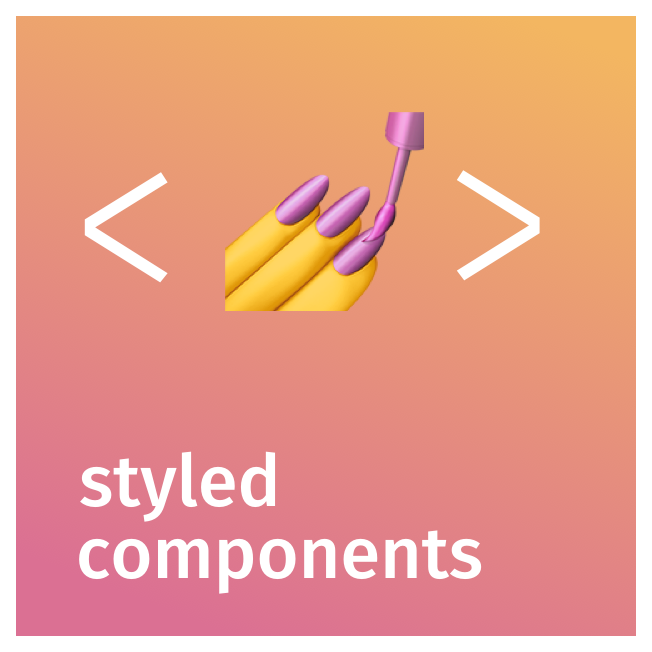
\includegraphics[height=2cm]{images/logos/styledComponent.png}
%     \caption{Logo de Styled Components}
% \end{figure}

\subsection*{TypeScript}
TypeScript est un langage de programmation open source qui étend la syntaxe de JavaScript en y ajoutant des fonctionnalités de typage statique. Il offre ainsi la possibilité de définir des types pour les variables, les paramètres de fonction, les objets et les valeurs de retour. Cette approche permet de détecter et de prévenir les erreurs de typage lors de la phase de développement, améliorant ainsi la robustesse et la qualité du code.
% \begin{figure}[!ht]
%     \centering %
%         
\includegraphics[height=2cm]{images/logos/typescript.png}
%     \caption{Logo de TypeScript}
% \end{figure}

\subsection*{Lerna}
Lerna est un outil open source qui facilite la gestion de projets monorepo, c'est-à-dire des projets qui contiennent plusieurs packages ou modules dans un même référentiel de code. Lerna permet de gérer ces packages de manière efficace en automatisant les tâches répétitives telles que l'installation des dépendances, la publication des packages, la gestion des versions, etc.\\

Avec Lerna, il est possible de partager du code entre différents packages, ce qui favorise la réutilisation et la modularité. Il permet également d'effectuer des tests et des déploiements cohérents sur l'ensemble des packages du monorepo.
% \begin{figure}[!ht]
%     \centering %
%         
\includegraphics[height=2cm]{images/logos/lerna.png}
%     \caption{Logo de Lerna}
% \end{figure}

\subsection*{Visual Studio Code}
Visual Studio Code est un éditeur de code extensible développé par Microsoft pour
Windows, Linux et macOS. Les fonctionnalités incluent la prise en charge du débogage,
la mise en évidence de la syntaxe, la complétion intelligente du code, les snippets, la
refactorisation du code et Git intégrer.
% \begin{figure}[!ht]
%     \centering %
%         
\includegraphics[height=2cm]{images/logos/vscode.jpeg}
%     \caption{Logo de Visual Studio Code}
% \end{figure}

\subsection*{IntelliJ IDEA}
IntelliJ IDEA, un environnement de développement intégré (IDE) puissant et polyvalent. IntelliJ IDEA est largement utilisé par les développeurs pour la programmation Java, mais il prend également en charge d'autres langages de programmation tels que JavaScript, TypeScript, Kotlin et bien d'autres.\\

IntelliJ IDEA offre une multitude de fonctionnalités pour améliorer la productivité des développeurs, telles que l'achèvement intelligent du code, la refactoring automatisé, la détection des erreurs en temps réel, la navigation avancée dans le code et bien d'autres. Il fournit également une intégration transparente avec les outils de gestion de version tels que Git, facilitant ainsi le suivi des modifications et la collaboration entre les membres de l'équipe.
% \begin{figure}[!ht]
%     \centering %
%         
\includegraphics[height=2cm]{images/logos/intellij logo.jpg}
%     \caption{Logo de IntelliJ}
% \end{figure}

\subsection*{Gradle}
\par Gradle est un moteur de production fonctionnant sur la plateforme Java. Il permet de construire des projets en Java, Scala, Groovy voire C++.

% \begin{figure}[!ht]
%     \centering %
%         
\includegraphics[height=2cm]{images/logos/gradle logo.png}
%     \caption{Logo de Gradle}
% \end{figure}

\par \textbf{Concepts de Gradle}
\begin{itemize}
\item  \textbf{Projets :}
Un projet représente une chose à faire, comme le déploiement d'applications dans des environnements de test. Un projet Gradle nécessite l'exécution d'un ensemble de tâches.

\item \textbf{Tâches :}
Une tâche fait référence à un travail effectué par un build. Cela peut être quelque chose d'aussi simple que compiler des classes, créer des fichiers JAR, créer Javadoc ou publier des archives.

\item  \textbf{Créer des scripts :}
Un script de construction est appelé build.gradle et se trouve dans le répertoire racine du projet. Chaque construction Gradle comprend un ou plusieurs projets.
\end{itemize}

\par \textbf{Fonctionnalités de Gradle}
\begin{itemize}
\item  \textbf{haute performance :}
Gradle termine rapidement la tâche en considérant les résultats des exécutions précédentes. Les travaux dont les entrées sont modifiées sont les seuls qui sont exécutés. Cela permet d'éviter les tâches inutiles et d'obtenir de meilleures performances.

\item  \textbf{Soutien :}
Connu pour fournir une assistance, nous utilisons Gradle pour les projets de construction ANT. Les tâches peuvent être importées depuis des projets de build ANT et peuvent être réutilisées dans Gradle. Il prend également en charge les dépôts Maven qui sont conçus pour publier et récupérer les dépendances du projet.

\item  \textbf{Construction de logiciel multi-projets :}
Gradle assure une prise en charge magnifique des builds multi-projets. Ces projets peuvent contenir un projet racine et un nombre illimité de sous-projets. Il prend en charge les constructions partielles, ce qui indique que l'outil déterminera si un projet dont notre projet dépend, a besoin d'un type de reconstruction. Au cas où le projet aurait besoin d'être reconstruit, Gradle le fera avant de construire d'autres projets.
\end{itemize}


\subsection*{Java}
Java est un langage populaire et largement utilisé dans le développement logiciel, notamment pour la création d'applications d'entreprise, de systèmes embarqués, de solutions web et bien plus encore.\\

Java offre de nombreux avantages, notamment sa portabilité, sa performance, sa sécurité et sa richesse en bibliothèques et frameworks. Il permet de développer des applications robustes et évolutives, en offrant une syntaxe claire et une structure orientée objet.

% \begin{figure}[!ht]
%     \centering %
%         
\includegraphics[height=2cm]{images/logos/java logo.png}
%     \caption{Logo de Java}
% \end{figure}

\subsection*{Java EE}
Java EE est une plateforme de développement d'applications d'entreprise qui fournit un ensemble de spécifications et de bibliothèques pour faciliter la création d'applications d'entreprise évolutives, robustes et sécurisées.\\

Java EE offre de nombreuses fonctionnalités et services essentiels pour le développement d'applications d'entreprise, tels que la gestion des transactions, la sécurité, la persistance des données, la gestion des ressources, la communication entre les composants et bien plus encore. Ces fonctionnalités intégrées permettent aux développeurs de se concentrer sur la logique métier de leur application, tout en bénéficiant d'une infrastructure solide et bien testée.
% \begin{figure}[!ht]
%     \centering %
%         
\includegraphics[height=2cm]{images/logos/java ee logo.png}
%     \caption{Logo de Java EE}
% \end{figure}

\subsection*{Spring}
Spring est un framework de développement d'applications Java qui offre une approche complète et modulaire pour la création d'applications d'entreprise.\\

Spring offre de nombreux modules et fonctionnalités qui facilitent le développement, tels que l'inversion de contrôle (IoC), la gestion des dépendances, la sécurité, la gestion des transactions, l'accès aux données, le développement web, et bien plus encore. Il favorise une architecture de développement propre et modulaire, permettant aux développeurs de se concentrer sur la logique métier de leur application sans se soucier des aspects techniques sous-jacents.
% \begin{figure}[!ht]
%     \centering %
%         
\includegraphics[height=2cm]{images/logos/spring logo.png}
%     \caption{Logo de Spring}
% \end{figure}

\subsection*{Sprign Boot}
Spring Boot est un framework basé sur Spring qui simplifie considérablement le processus de création d'applications Java autonomes et prêtes à l'emploi.\\

Spring Boot facilite la configuration et le déploiement de l'application en fournissant des conventions par défaut et en minimisant la configuration manuelle. Il offre également une intégration transparente avec d'autres technologies et frameworks, ce qui permet de développer rapidement des applications robustes.
% \begin{figure}[!ht]
%     \centering %
%         
\includegraphics[height=2cm]{images/logos/spring boot logo.png}
%     \caption{Logo de Spring Boot}
% \end{figure}

\subsection*{Sprign Security}
Spring Security est un framework puissant qui fournit des fonctionnalités de sécurité avancées pour les applications Java.\\

Avec Spring Security, nous avons pu mettre en place une authentification et une autorisation robustes pour nos utilisateurs. Nous avons utilisé différents mécanismes d'authentification, tels que l'authentification basée sur des formulaires, l'authentification basée sur des jetons, ainsi que l'intégration avec des fournisseurs d'authentification externes tels que OAuth.
% \begin{figure}[!ht]
%     \centering %
%         
\includegraphics[height=2cm]{images/logos/spring boot logo.png}
%     \caption{Logo de Spring Boot}
% \end{figure}


\subsection*{Pebble}
Pebble est un moteur de templates Java léger et puissant qui facilite la création de vues dynamiques et réutilisables.\\

Grâce à Pebble, nous avons pu séparer la logique métier de la présentation en utilisant des templates. Les templates Pebble sont écrits en utilisant une syntaxe simple et intuitive, ce qui nous a permis de créer rapidement des vues attrayantes et réactives pour notre application.

% \begin{figure}[!ht]
%     \centering %
%         
\includegraphics[height=2cm]{images/logos/pebble logo.png}
%     \caption{Logo de Pebble}
% \end{figure}

\subsection*{Jolt}
Jolt est un outil puissant qui nous a permis de structurer et de manipuler facilement des données JSON complexes.\\

Avec Jolt, nous avons pu définir des spécifications de transformation JSON en utilisant un langage de configuration simple et concis. Ces spécifications décrivent les modifications souhaitées dans la structure et les valeurs des données JSON, permettant ainsi de les transformer selon nos besoins.

% \begin{figure}[!ht]
%     \centering %
%         
\includegraphics[height=2cm]{images/logos/jolt_logo.png}
%     \caption{Logo de Jolt}
% \end{figure}

\subsection*{GraphQL}
GraphQL est un langage de requête et une technologie de communication de données qui offre une approche flexible et efficace pour récupérer et manipuler des données. Dans notre projet, nous avons utilisé GraphQL pour mettre en place une API de données robuste et personnalisable.\\

Avec GraphQL, nous avons pu définir un schéma de données qui décrit les types et les relations entre les données. Ce schéma agit comme un contrat entre le client et le serveur, permettant au client de spécifier exactement les données dont il a besoin et de les récupérer en une seule requête. Cela évite les problèmes de surcharge de données et d'appels multiples à l'API, améliorant ainsi les performances et l'efficacité.
% \begin{figure}[!ht]
%     \centering %
%         
\includegraphics[height=2cm]{images/logos/graphql logo.png}
%     \caption{Logo de GraphQL}
% \end{figure}

\subsection*{JUnit}
JUnit est un framework de test unitaire pour le langage de programmation Java. Dans notre projet, nous avons utilisé JUnit pour effectuer des tests unitaires afin de vérifier le bon fonctionnement de nos classes et méthodes individuelles.\\

JUnit offre une structure de test simple et efficace, permettant aux développeurs de définir des cas de test et d'exécuter automatiquement ces tests. Il fournit des assertions pour vérifier les résultats attendus des différentes opérations, ce qui facilite la détection des erreurs et des bugs.
% \begin{figure}[!ht]
%     \centering %
%         
\includegraphics[height=2cm]{images/logos/junit logo.png}
%     \caption{Logo de JUnit}
% \end{figure}


\subsection{Outils de documentation}
\subsection*{Storybook}
Storybook est un outil de développement interactif et de documentation qui facilite la création,
le test et la documentation des composants d’interface utilisateur. Il permet aux développeurs
de concevoir et de visualiser les composants de manière isolée, ce qui facilite l’exploration et la
validation des différentes configurations. Grâce à son interface intuitive, Storybook simplifie le
processus de développement et de débogage des composants. Il favorise également la collaboration
en permettant le partage des composants et la génération automatique de documentation. En
résumé, Storybook améliore l’efficacité du développement en offrant un environnement interactif
pour le développement et la documentation des composants d’interface utilisateur.
% \begin{figure}[!ht]
%     \centering %
%         
\includegraphics[height=2cm]{images/logos/storyboojk.png}
%     \caption{Logo de Storybook}
% \end{figure}

\subsection*{Swagger}
Swagger est un ensemble d'outils open-source permettant de concevoir, de construire, de documenter et de consommer des API RESTful. Il offre une approche basée sur la spécification, ce qui permet de décrire l'ensemble des fonctionnalités d'une API de manière standardisée et compréhensible par les développeurs et les utilisateurs.\\

Le cœur de Swagger est la spécification OpenAPI, anciennement connue sous le nom de Swagger Specification. Cette spécification utilise le format JSON ou YAML pour décrire les endpoints, les paramètres, les réponses et d'autres éléments clés d'une API. Grâce à cette spécification, il devient possible de générer automatiquement de la documentation interactive, des SDKs clients, des tests automatisés et d'autres artefacts liés à l'API.
% \begin{figure}[!ht]
%     \centering %
%         
\includegraphics[height=2cm]{images/logos/swagger.png}
%     \caption{Logo de Swagger}
% \end{figure}


\subsection{Outils de Test}
\subsection*{Cypress}
Cypress est un outil de test d'interface utilisateur open source, utilisé pour effectuer des tests end-to-end sur des applications web. Il offre une approche moderne et efficace pour écrire et exécuter des tests fonctionnels, intégration et de bout en bout.\\

Cypress se distingue par sa simplicité d'utilisation et sa capacité à exécuter les tests directement dans le navigateur. Il permet aux développeurs d'écrire des tests en utilisant une syntaxe JavaScript familière, et offre une interface de test interactive qui facilite le débogage et l'inspection des éléments de l'application.
% \begin{figure}[!ht]
%     \centering %
%         
\includegraphics[height=2cm]{images/logos/cypress.jpeg}
%     \caption{Logo de Cypress}
% \end{figure}

\subsection*{Postman}
Postman est un outil populaire utilisé pour tester et développer des API. Il offre une interface conviviale qui permet aux développeurs de créer, envoyer et analyser des requêtes HTTP à destination de différentes API.\\

Dans notre projet, nous avons utilisé Postman pour tester et valider nos API. Nous avons pu envoyer des requêtes GET, POST, PUT, DELETE, etc. vers nos points de terminaison d'API pour vérifier leur fonctionnement et leur conformité aux spécifications.
% \begin{figure}[!ht]
%     \centering %
%         
\includegraphics[height=2cm]{images/logos/postmanLogo.png}
%     \caption{Logo de Postman}
% \end{figure}

\subsection*{SoapUI}
SOAPUI est un outil open-source utilisé pour tester les services Web basés sur le protocole SOAP (Simple Object Access Protocol). Il offre une interface conviviale permettant de créer, exécuter et analyser des tests automatisés pour les services Web.\\

Avec SOAPUI, les développeurs et les testeurs peuvent facilement créer des requêtes SOAP en spécifiant les paramètres et les en-têtes appropriés. Ils peuvent également configurer des assertions pour valider les réponses des services en vérifiant les valeurs, les codes de statut et d'autres critères prédéfinis.
% \begin{figure}[!ht]
%     \centering %
%         
\includegraphics[height=2cm]{images/logos/soapui.png}
%     \caption{Logo de SoapUI}
% \end{figure}

\subsection*{Karate}
Karate est un framework open-source de test d'API qui prend en charge les tests automatisés de services Web REST et SOAP. Il offre une approche simple et expressive pour écrire des scénarios de test, en utilisant un langage de script spécifique à Karate basé sur le langage Gherkin.\\

Avec Karate, les développeurs et les testeurs peuvent définir des étapes de test déclaratives dans des fichiers de scénarios, en utilisant des mots-clés compréhensibles par les acteurs métier. Cela permet de créer des tests automatisés faciles à comprendre et à maintenir, sans nécessiter de connaissances approfondies en programmation.
% \begin{figure}[!ht]
%     \centering %
%         
\includegraphics[height=2cm]{images/logos/karate logo.png}
%     \caption{Logo de Karate}
% \end{figure}

\subsection*{Gherkin}
Le langage Gherkin est un langage utilisé pour écrire des scénarios de tests automatisés, basés sur le comportement attendu du système. Il se distingue par sa lisibilité et sa simplicité, ce qui le rend accessible aux acteurs métier non techniques.\\

Gherkin est basé sur une syntaxe claire et structurée, utilisant des mots-clés spécifiques tels que "Given" (Étant donné), "When" (Quand), "Then" (Alors) et d'autres. Ces mots-clés permettent de décrire les différentes étapes d'un scénario et d'exprimer les attentes vis-à-vis du système.
% \begin{figure}[!ht]
%     \centering %
%         
\includegraphics[height=2cm]{images/logos/gherkin.png}
%     \caption{Logo de Gherkin}
% \end{figure}


\subsection{Outils de Gestion de Version}
\subsection*{Github}
GitHub, en tant qu’outil essentiel dans le développement front-end, joue un rôle central dans la
gestion de version et la collaboration. Il permet un contrôle précis des modifications du code source,
des revues de code efficaces et une intégration fluide des fonctionnalités développées. GitHub assure
la qualité, la traçabilité et la cohérence du travail tout au long du projet.
% \begin{figure}[!ht]
%     \centering %
%         
\includegraphics[height=2cm]{images/logos/github.png}
%     \caption{Logo de Github}
% \end{figure}

\subsection{Outils de DevOps}
\subsection*{Intégration continue}
\subsubsection*{Sonarqube}
Sonarqube enregistre les mesures de qualité dans une base de données et les présente dans un tableau de
bord. Il fournit des tendances et des indicateurs avancés. L’idée principale est de fournir à
chaque développeur les mesures de la qualité du code de leurs projets.
% \begin{figure}[!ht]
%     \centering %
%         
\includegraphics[height=2cm]{images/logos/sonarqube_logo.jpg}
%     \caption{Logo de Sonarqube}
% \end{figure}

\subsubsection*{Bolt-CI}
Une solution interne qui se charge des builds et des tests et qui informe les développeurs de
l’état de leur travail par mail ou dans leur profil github à chaque commit, dans les 2 premières
minutes après avoir déposé le code dans le repository. Elle informe également les autres outils
des changements dans les repositories github.\\

Une solution interne qui se charge de l’automatisation des builds et des tests (principalement
les tests unitaires), et qui renvoie le feedback aux développeurs par mail et github, après chaque
pull request fusionée.
% \begin{figure}[!ht]
%     \centering %
%         
\includegraphics[height=2cm]{images/logos/boltCI-logo.png}
%     \caption{Logo de Bolt-CI}
% \end{figure}


\subsection*{Livraison continue}
\subsubsection*{Jenkins}
Jenkins est un outil d’automatisation open-source écrit en Java avec des plugins construits pour
les besoins du livraison continue. Jenkins est utilisé pour builder et tester vos projets logiciels
en temps réel, ce qui permet aux développeurs d’intégrer plus facilement les modifications
apportées au projet et aux utilisateurs d’obtenir plus facilement une nouvelle version.
% \begin{figure}[!ht]
%     \centering %
%         
\includegraphics[height=2cm]{images/logos/jenkins-logo.png}
%     \caption{Logo de Jenkins}
% \end{figure}


\subsubsection*{Nexus}
Ce gestionnaire de dépôt permet de stocker et de récupérer des artefacts de
build. Il s’agit d’une version privée similaire aux gestionnaires de dépôts publics
populaires comme Maven Central Repository et jcenter de Bintray, que tout le
monde peut utiliser pour récupérer les dépendances publiques pour un projet
Maven.
% \begin{figure}[!ht]
%     \centering %
%         
\includegraphics[height=2cm]{images/logos/nexus-logo.png}
%     \caption{Logo de Nexus}
% \end{figure}

\subsection*{Déploiement}
\subsubsection*{Bolt}
Il s’agit d’un outil développé en interne et fonctionnant dans tous les nœuds des machines
virtuelles de notre infrastructure. Il fournit une interface de ligne de commande simple pour
déclencher l’exécution de divers types d’applications avec une syntaxe à la fois simple et puissante.
% \begin{figure}[!ht]
%     \centering %
%         
\includegraphics[height=2cm]{images/logos/boltCI-logo.png}
%     \caption{Logo de Bolt}
% \end{figure}

\subsubsection*{Nomad}
HashiCorp Nomad est un gestionnaire de charge moderne et léger. Nomad est également
connu comme un moteur d’orchestration comme Kubernetes. HashiCorp Nomad permet à toute organisation de déployer et de gérer facilement ses applications. Il peut non seulement orchestrer des applications conteneurisées mais aussi des applications patrimoniales à l’aide d’un flux de travail unique et unifié. Nomad peut également exécuter des applications Docker, non conteneurisées, microservices et batch.
% \begin{figure}[!ht]
%     \centering %
%         
\includegraphics[height=2cm]{images/logos/nomad-logo.png}
%     \caption{Logo de Nomad}
% \end{figure}

\subsubsection*{Consul}
Consul est solution utilisée pour configurer dynamiquement des applications, coordonner des services,
ou servir de back-end de données pour Vault, ainsi qu’une multitude d’autres utilisations.
% \begin{figure}[!ht]
%     \centering %
%         
\includegraphics[height=2cm]{images/logos/consul-logo.png}
%     \caption{Logo de Consul}
% \end{figure}

\subsubsection*{Vault}
Vault est un système de gestion des secrets et du chiffrement. Un secret est toute chose
dont on souhaite contrôler strictement l’accès, comme les clés de chiffrement des API, les mots de passe ou les certificats. Vault fournit des services de cryptage qui sont contrôlés par des méthodes d’authentification et d’autorisation. À l’aide de l’interface utilisateur, de l’interface
CLI ou de l’API HTTP de Vault, l’accès aux secrets et à d’autres données sensibles peut être
stocké et géré en toute sécurité, rigoureusement contrôlé (restreint) et vérifiable.
% \begin{figure}[!ht]
%     \centering %
%         
\includegraphics[height=2cm]{images/logos/vault-logo.png}
%     \caption{Logo de Vault}
% \end{figure}

\subsection{Outils de Routage}
\subsection*{VIP}
Une VIP \textbf{adresse IP virtuelle} (ou VIPA) est une adresse IP publique qui
peut être partagée par plusieurs appareils connectés. En interne, chaque appareil
possède une adresse IP locale unique, mais en externe, ils partagent tous la même
adresse IP.

\subsection*{Traefik}
Traefik est un reverse proxy/load balancer. en tant que reverse proxy Traefik facilite le déploiement de micro-services. Il nous fournit un point d’entrée commun
vers notre infrastructure et permet de suivre et de surveiller toutes les requêtes entrantes et sortantes, et en tant que load balancer traefik peut distribuer la charge
sur tous les instances de notre système.
% \begin{figure}[!ht]
%     \centering %
%         
\includegraphics[height=2cm]{images/logos/traefik-logo.png}
%     \caption{Logo de Traefik}
% \end{figure}

\subsection{Outils de Monitoring}
\subsection*{Grafana}
Au sein de la DiFa, garantir la disponibilité des services informatique est primordiale, pour cela l’équipe a pris une décision pour utiliser grafana comme étant un
outil de reporting, en effet grafana est une plateforme open source taillée pour
la surveillance, l’analyse et la visualisation des métriques. Elle est livrée avec un
serveur web (écrit en Go) permettant d’y accéder via une API HTTP.
% \begin{figure}[!ht]
%     \centering %
%         
\includegraphics[height=2cm]{images/logos/grafana.jpg}
%     \caption{Logo de Grafana}
% \end{figure}

\subsection*{Kibana}
Pour mettre les logs visible est simple a comprendre, la DiFa a decidé d’utiliser
Kibana qui est est une application frontend gratuite et ouverte qui s’appuie sur la
Suite Elastic. Elle permet de rechercher et de visualiser les données indexées dans
Elasticsearch.Elle sert aussi d’interface utilisateur pour le monitoring, la gestion
et la sécurité des clusters de la Suite Elastic.
% \begin{figure}[!ht]
%     \centering %
%         
\includegraphics[height=2cm]{images/logos/kibana.png}
%     \caption{Logo de Kibana}
% \end{figure}

\section{Interfaces}
Dans cette section consacrée à l'interface de notre application de banque en ligne, nous présentons les différentes pages et fonctionnalités qui permettent aux utilisateurs de gérer leurs comptes bancaires de manière pratique et personnalisée. Nous avons développé des interfaces adaptées à différents types d'appareils, notamment le bureau, la tablette et le mobile, afin d'offrir une expérience utilisateur optimale sur chaque plateforme.\\

Nous avons pris en compte les préférences linguistiques des utilisateurs en proposant des versions de langue en français et en anglais pour toutes les interfaces. Cela permet aux utilisateurs de choisir la langue qui leur convient le mieux, facilitant ainsi leur compréhension et leur interaction avec l'application, quel que soit leur pays ou leur langue préférée.
\subsection{Accueil}
Cette page constitue le point d'entrée principal pour les utilisateurs et offre une expérience conviviale et intuitive. Elle propose plusieurs options et fonctionnalités pour répondre aux besoins des utilisateurs.\\

Sur la page d'accueil, les utilisateurs ont la possibilité de choisir parmi différentes actions, telles que se connecter à leur compte, s'inscrire en tant que nouveau client, accéder au mode démonstration pour découvrir les fonctionnalités de l'application, utiliser le simulateur de crédit pour estimer les possibilités de financement, consulter les questions fréquentes pour obtenir des réponses aux interrogations courantes, trouver une agence bancaire à proximité, consulter les taux de change actuels et contacter notre équipe d'assistance via le formulaire de contact.
\begin{figure}[!ht]
    \centering
    \begin{subfigure}[b]{0.49\textwidth}
        \centering
        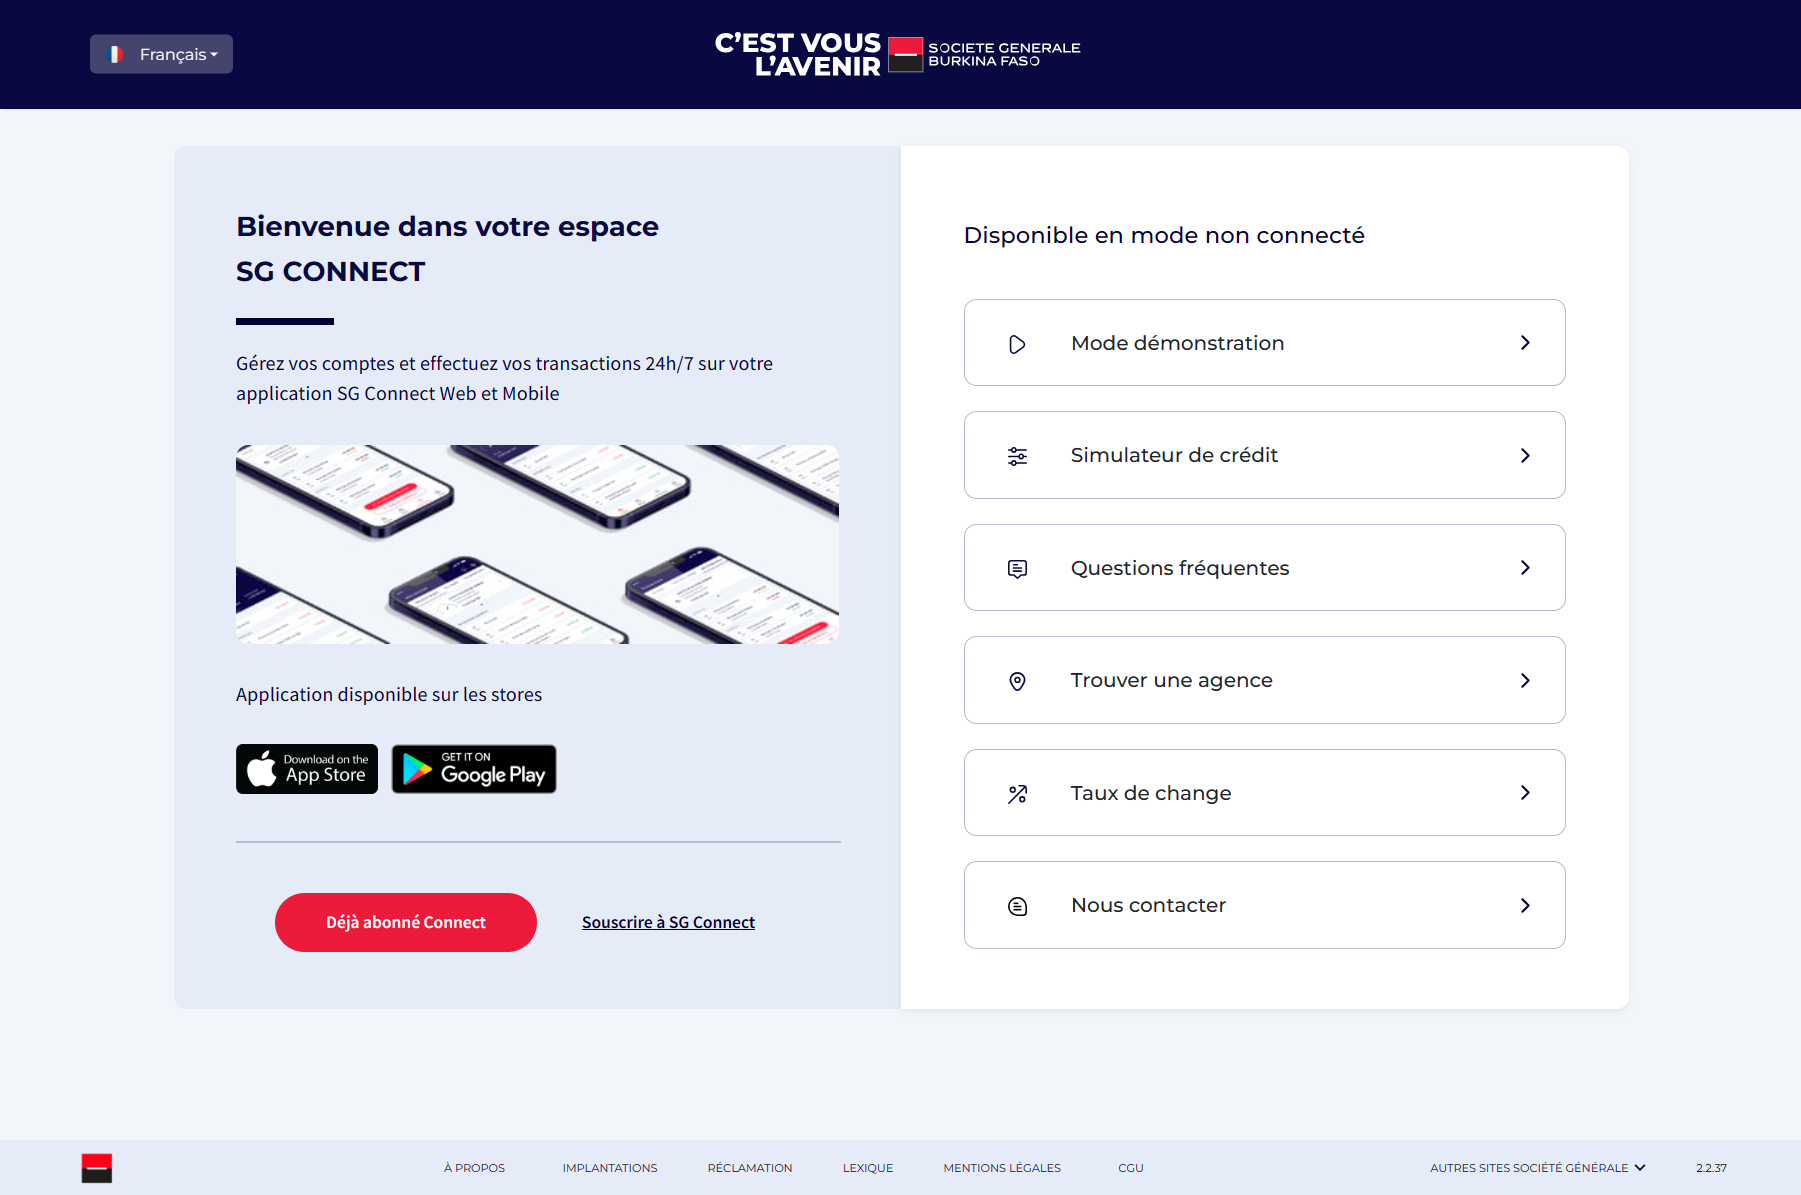
\includegraphics[width=\textwidth]{images/screens/accueil/desktop.png}
        \caption{version française}
    \end{subfigure}
    \hfill
    \begin{subfigure}[b]{0.49\textwidth}
        \centering
        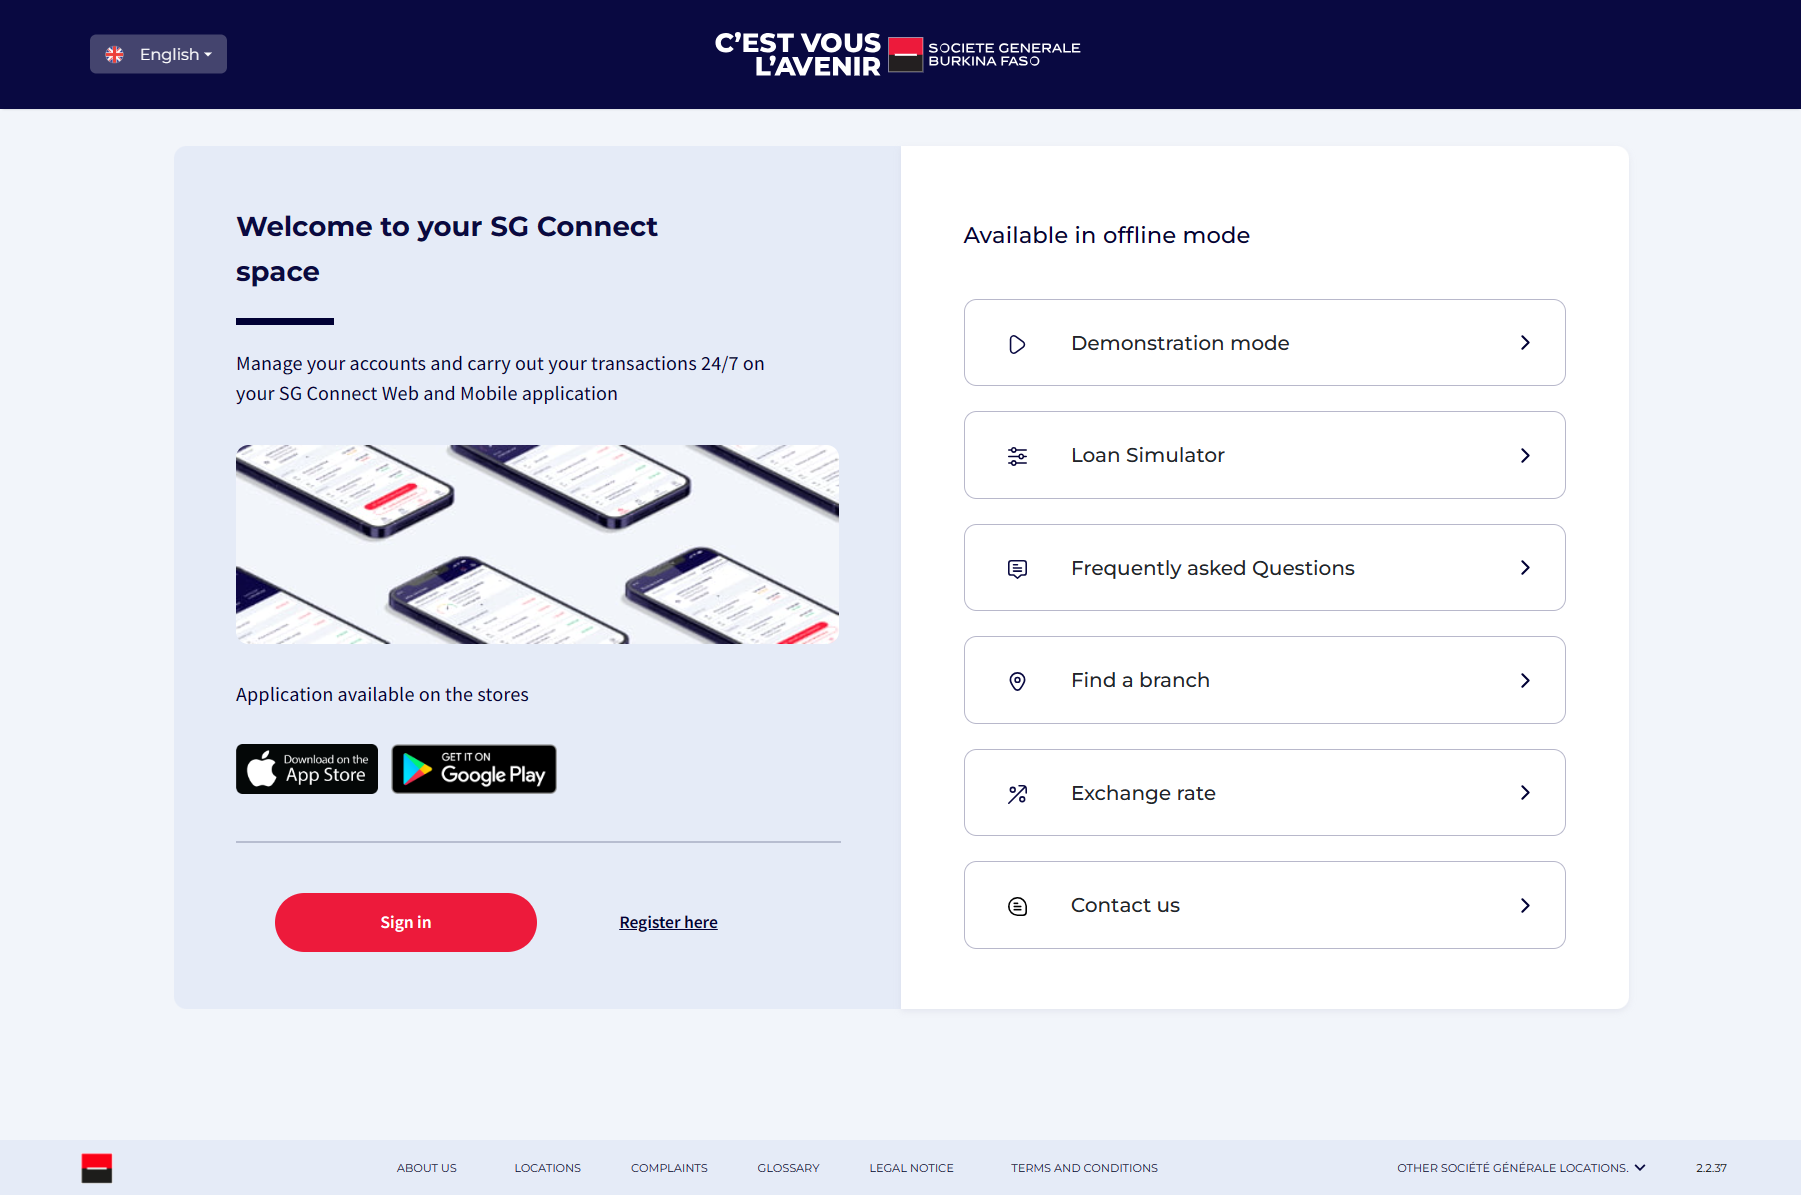
\includegraphics[width=\textwidth]{images/screens/home/desktop.png}
        \caption{version anglaise}
    \end{subfigure}
       \caption{Interface Accueil sur le bureau}
\end{figure}

\newpage

\begin{figure}[!h]
    \centering
    \begin{subfigure}[b]{0.49\textwidth}
        \centering
        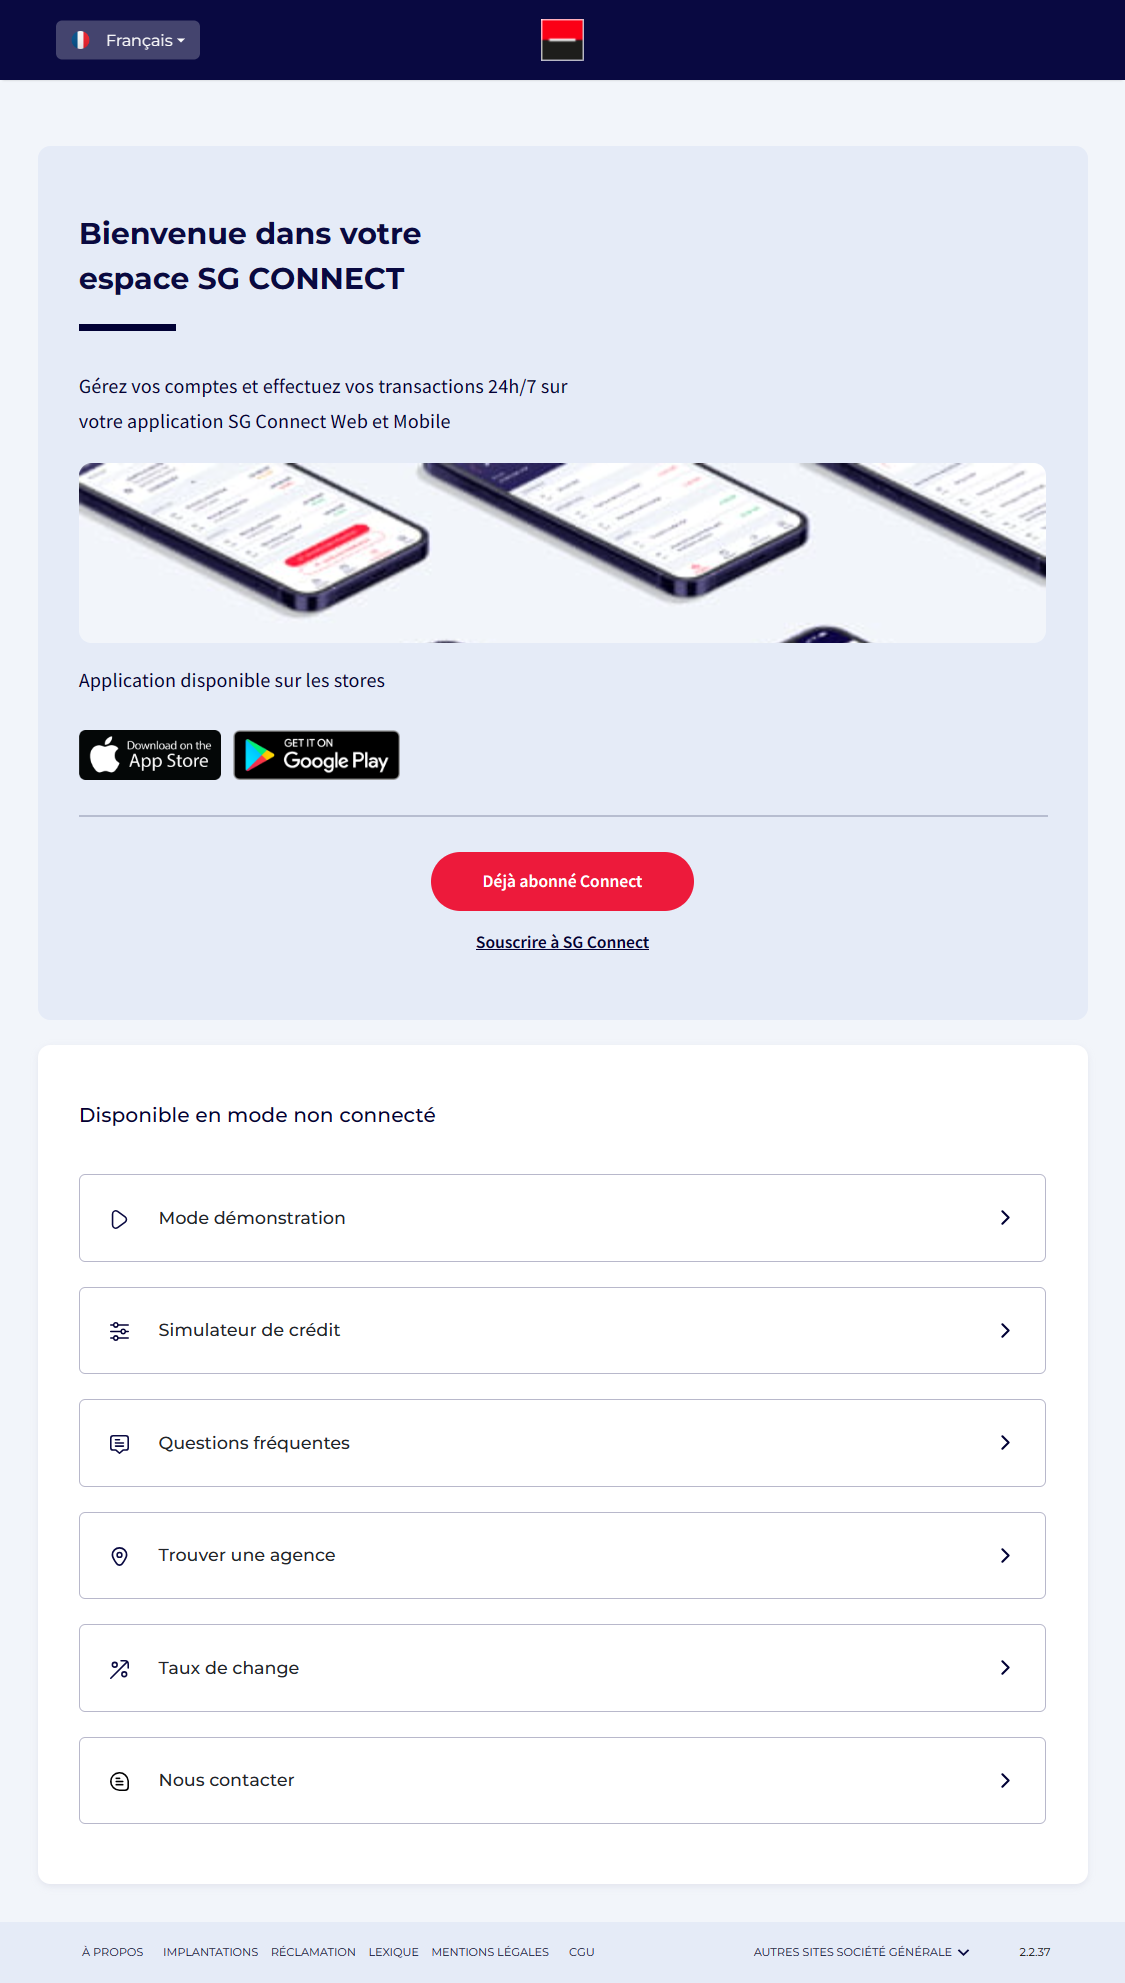
\includegraphics[width=\textwidth]{images/screens/accueil/tablette.png}
        \caption{version française}
    \end{subfigure}
    \hfill
    \begin{subfigure}[b]{0.49\textwidth}
        \centering
        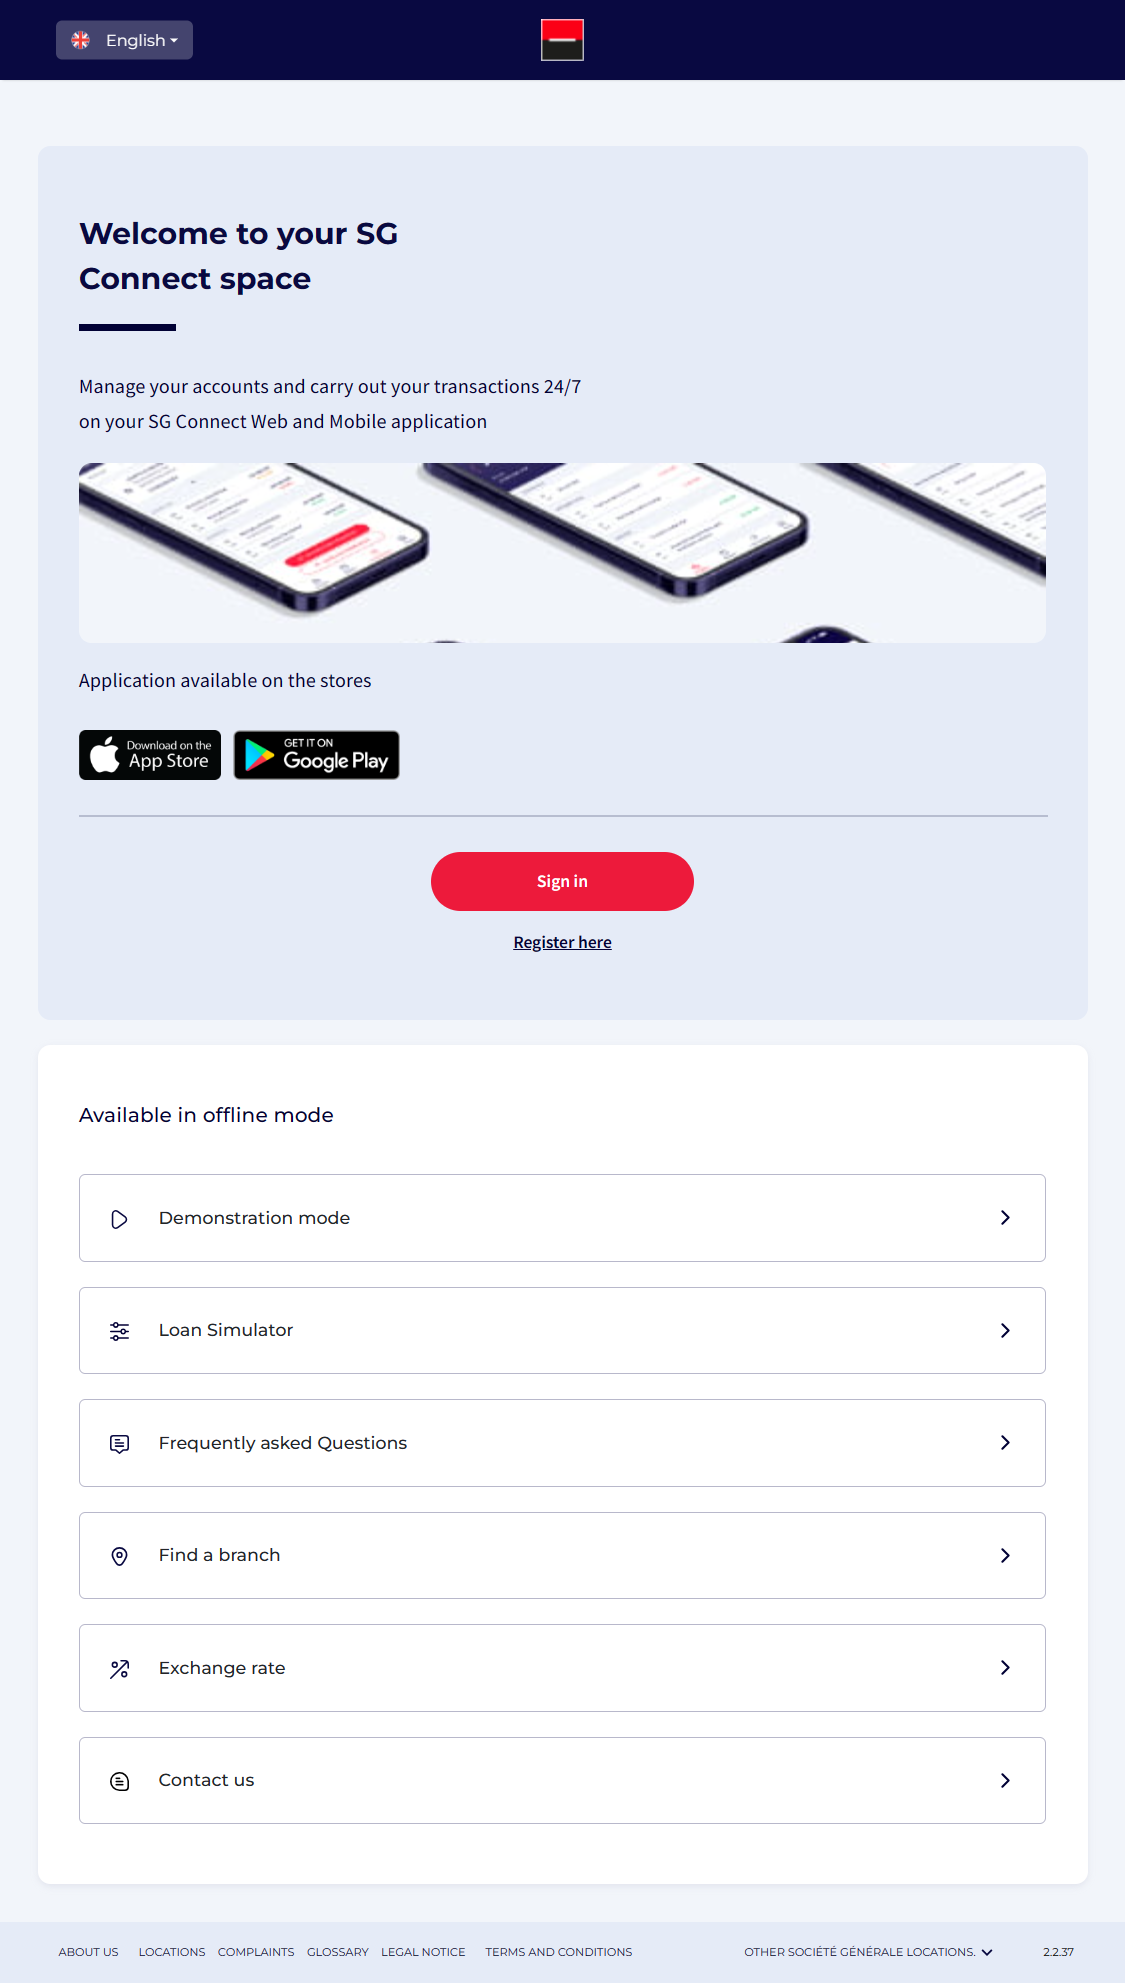
\includegraphics[width=\textwidth]{images/screens/home/tablette.png}
        \caption{version anglaise}
    \end{subfigure}
       \caption{Interface Accueil sur la tablette}
\end{figure}

\newpage

\begin{figure}[!ht]
    \centering
    \begin{subfigure}[b]{0.49\textwidth}
        \centering
        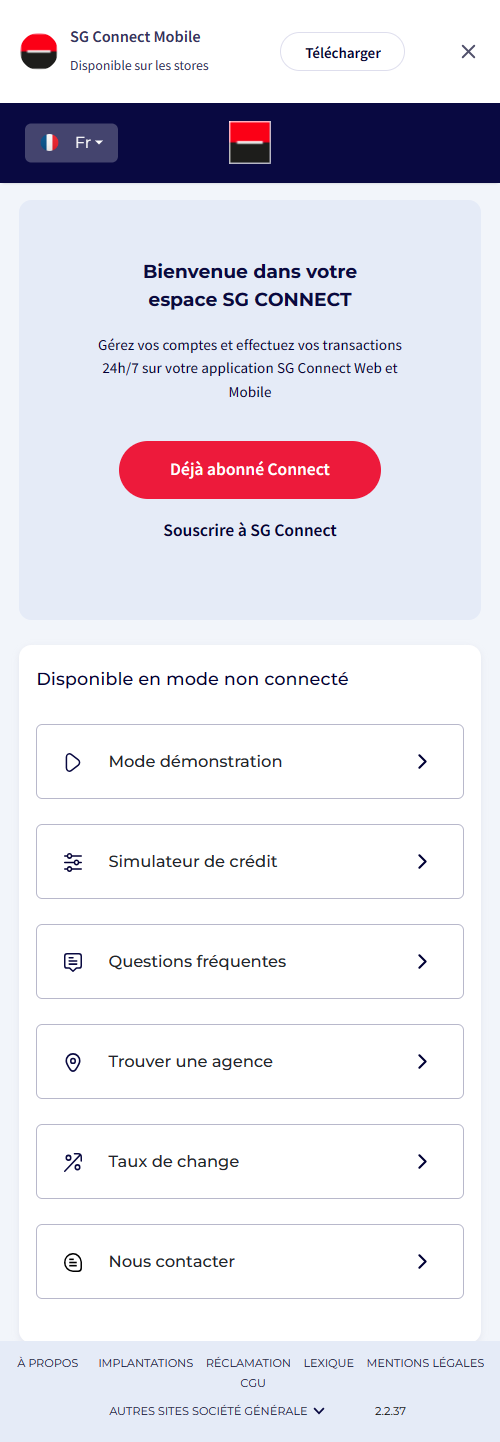
\includegraphics[width=\textwidth]{images/screens/accueil/mob.png}
        \caption{version française}
    \end{subfigure}
    \hfill
    \begin{subfigure}[b]{0.49\textwidth}
        \centering
        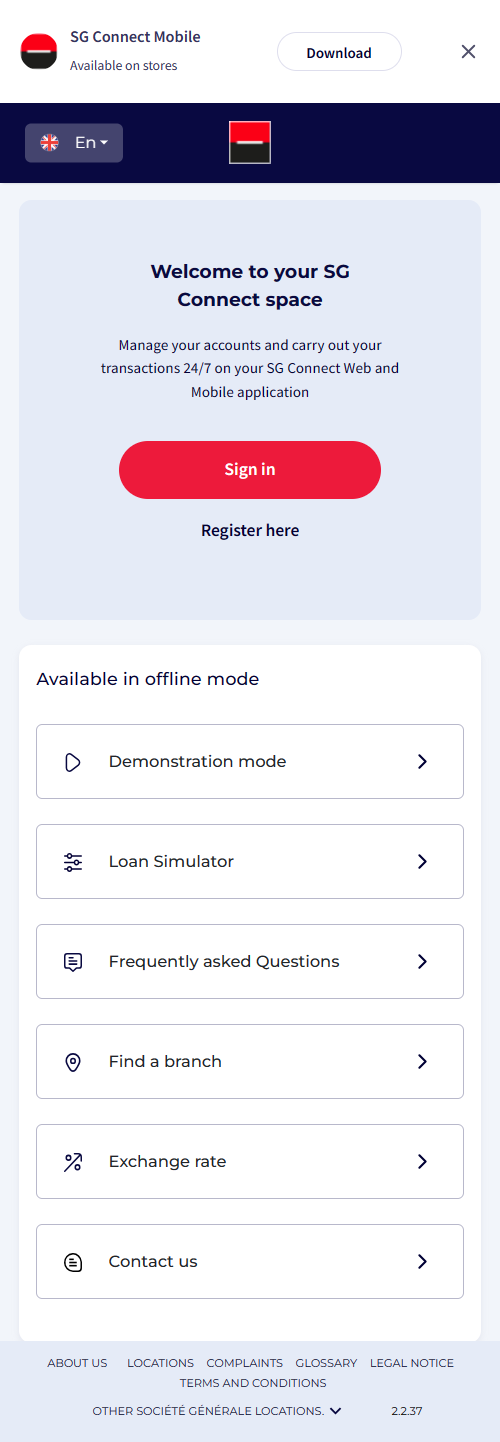
\includegraphics[width=\textwidth]{images/screens/home/mob.png}
        \caption{version anglaise}
    \end{subfigure}
       \caption{Interface Accueil sur le mobile}
\end{figure}

\newpage

\subsection{Changement de langue}
Ce bouton permet aux utilisateurs de sélectionner la langue de leur choix pour afficher le contenu de l'application dans cette langue spécifique. Lorsque l'utilisateur clique sur le bouton de changement de langue, une alerte s'affiche avec deux options : confirmation et annulation.\\

Si l'utilisateur choisit de confirmer le changement de langue, l'application effectue le changement et redirige l'utilisateur vers la page d'accueil dans la nouvelle langue sélectionnée. Cela lui permet de bénéficier d'une expérience utilisateur dans la langue de son choix.\\

D'autre part, si l'utilisateur choisit d'annuler le changement de langue, aucun changement ne sera effectué et il restera sur la même page dans la langue actuelle.
\begin{figure}[!ht]
    \centering %
        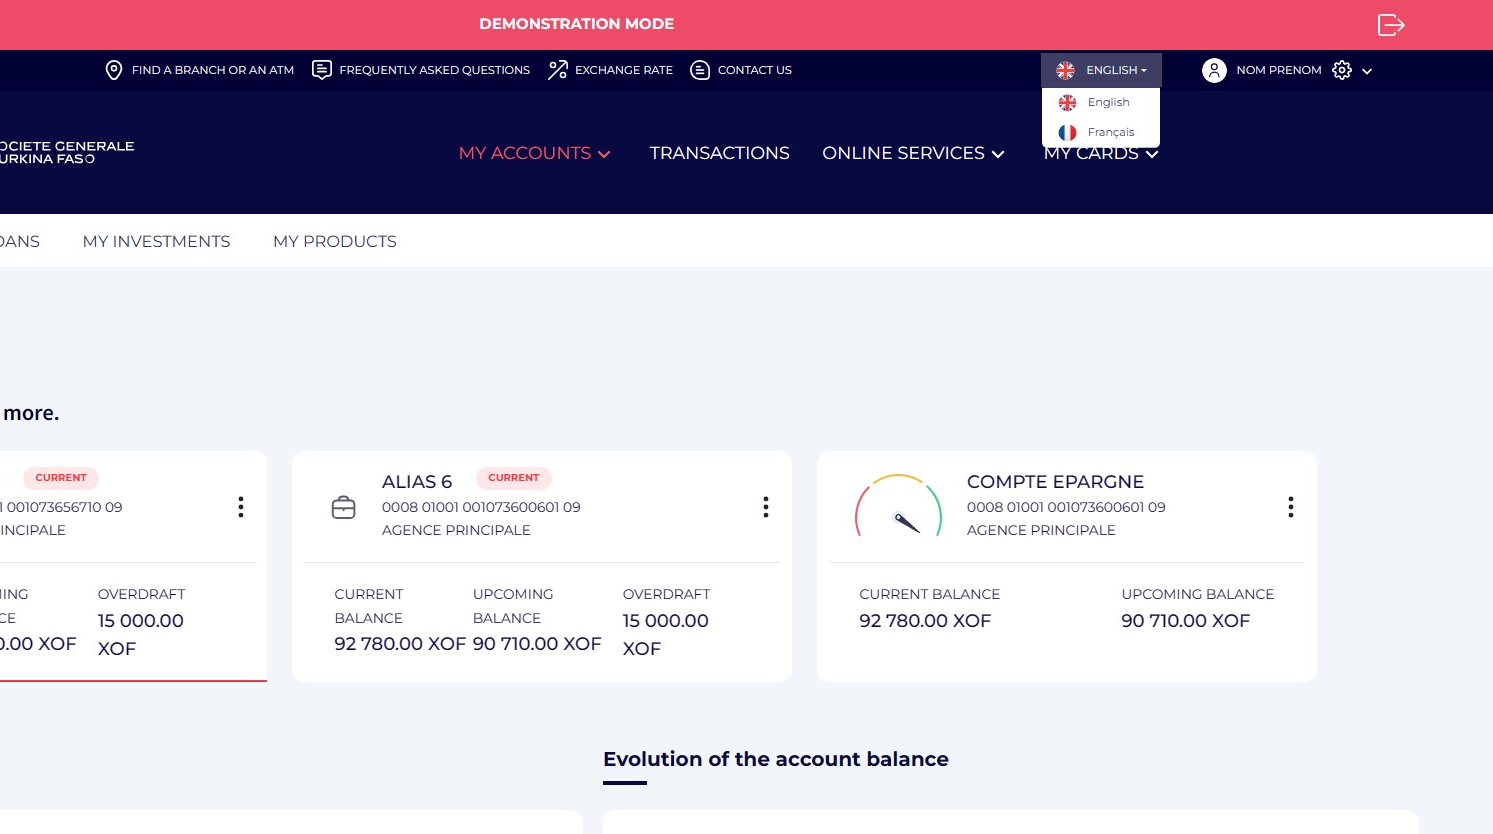
\includegraphics[width=16cm]{images/screens/switch/desktop-switch.png}
    \caption{Bouton de changement de langue}
\end{figure}

\begin{figure}[!ht]
    \centering
    \begin{subfigure}[b]{0.49\textwidth}
        \centering
        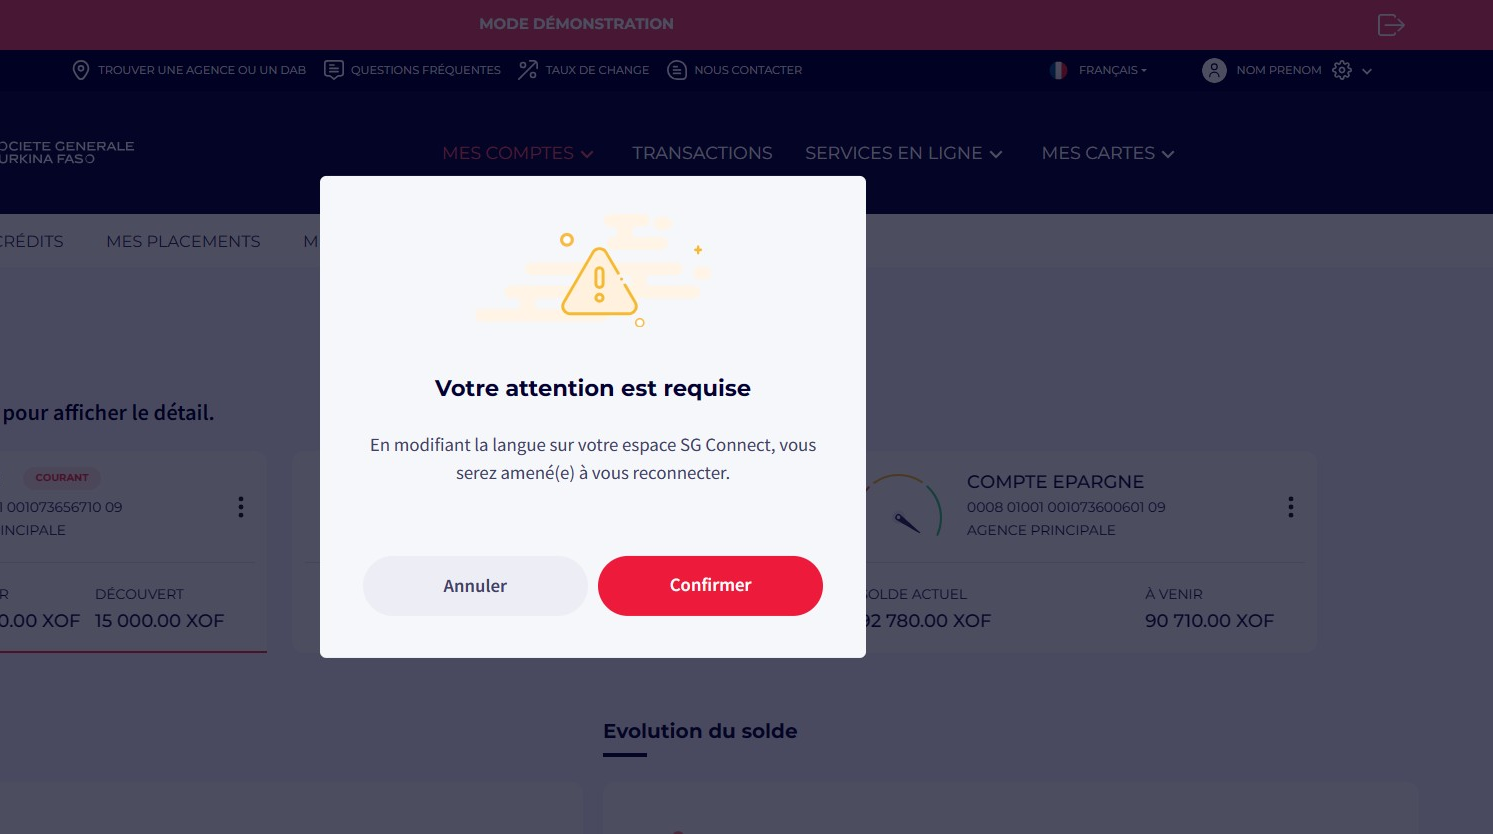
\includegraphics[width=\textwidth]{images/screens/switch/desktop-fr.png}
        \caption{version française}
    \end{subfigure}
    \hfill
    \begin{subfigure}[b]{0.49\textwidth}
        \centering
        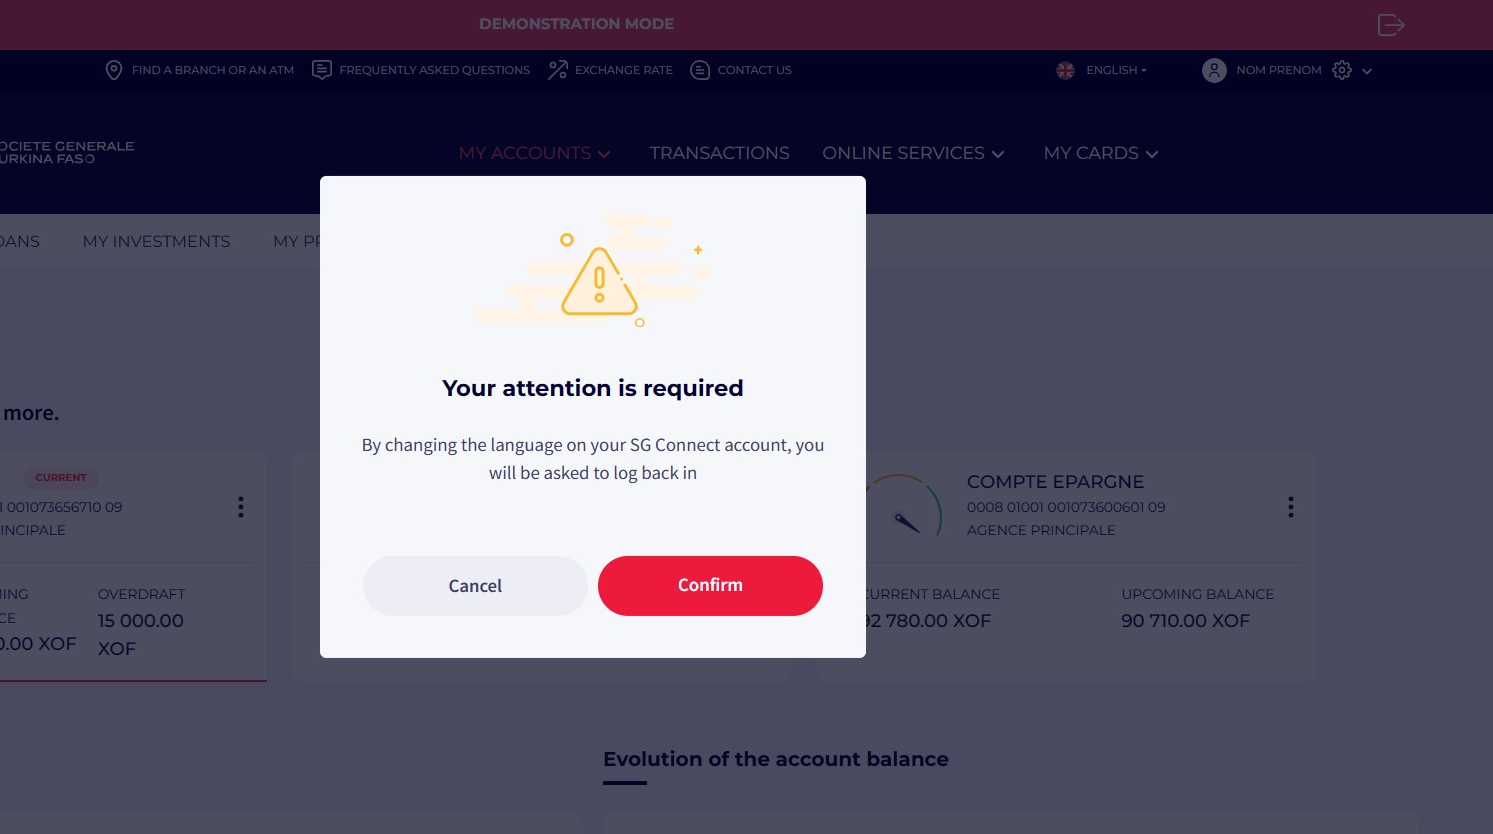
\includegraphics[width=\textwidth]{images/screens/switch/desktop-ang.png}
        \caption{version anglaise}
    \end{subfigure}
       \caption{Alerte de changement de langue sur le bureau et la tablette}
\end{figure}
\newpage

\begin{figure}[!ht]
    \centering
    \begin{subfigure}[b]{0.49\textwidth}
        \centering
        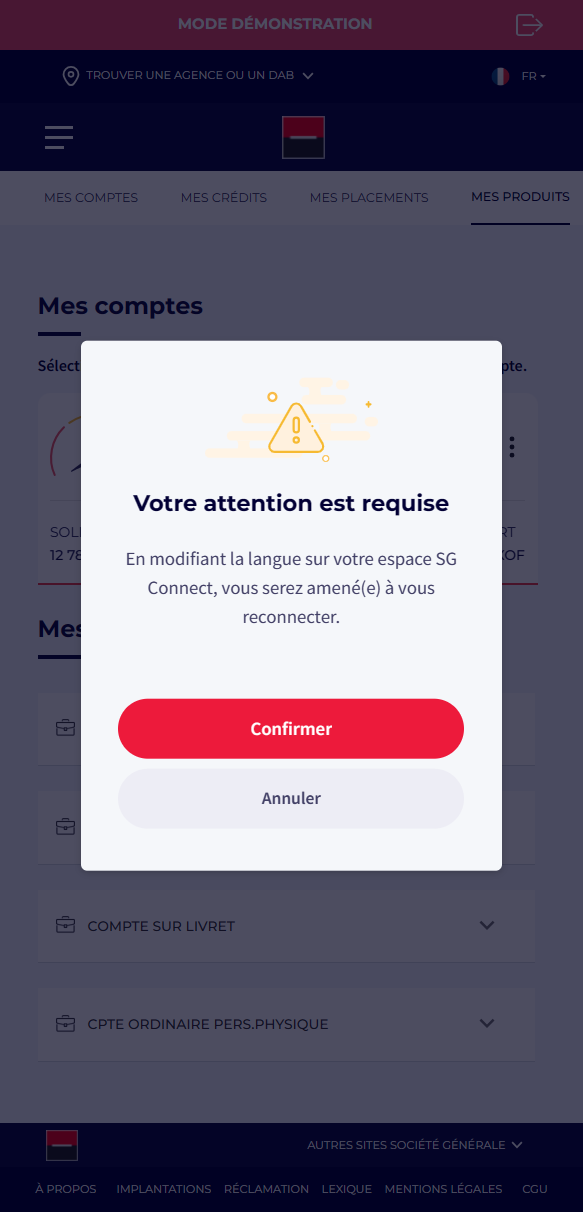
\includegraphics[width=\textwidth]{images/screens/switch/mob-fr.png}
        \caption{version française}
    \end{subfigure}
    \hfill
    \begin{subfigure}[b]{0.49\textwidth}
        \centering
        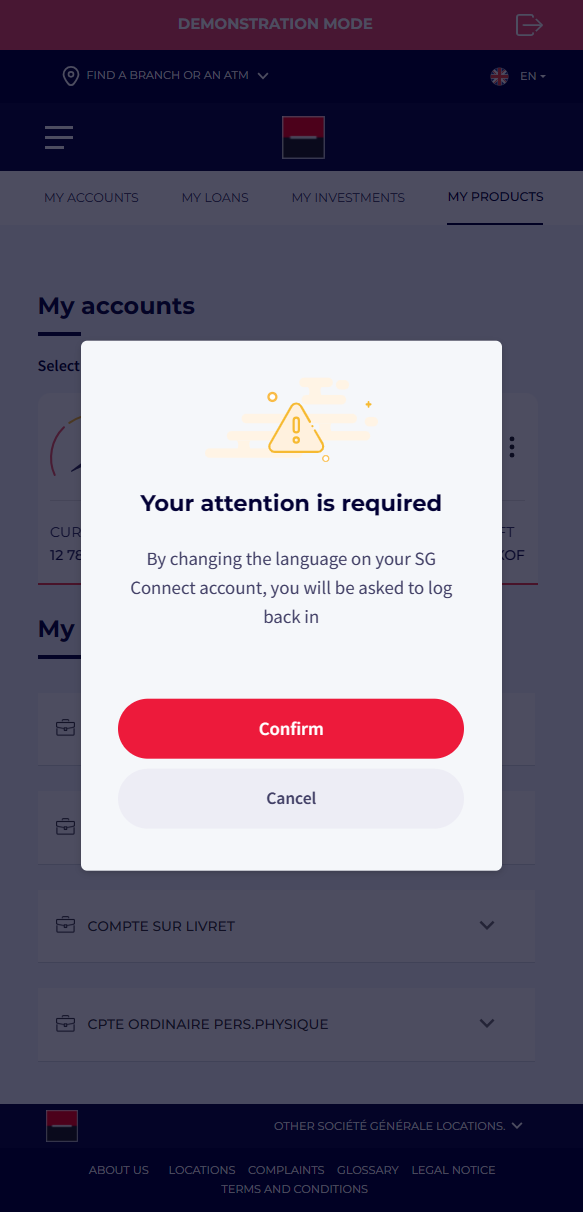
\includegraphics[width=\textwidth]{images/screens/switch/mob-ang.png}
        \caption{version anglaise}
    \end{subfigure}
       \caption{Alerte de changement de langue sur le mobile}
\end{figure}

\subsection{Mes Cartes}
L'interface "Mes cartes" offre une présentation claire et organisée des cartes monétiques, en fournissant des informations détaillées telles que le type de carte, le numéro de carte et la date d'expiration. Les utilisateurs peuvent également accéder à l'historique complet des transactions effectuées avec chaque carte, leur permettant ainsi de suivre leurs dépenses et de détecter les transactions suspectes. Cette interface utilise les API \textbf{getCards} et \textbf{getCardTransactions} pour récupérer les données nécessaires.
\begin{figure}[!ht]
    \centering
    \begin{subfigure}[b]{0.49\textwidth}
        \centering
        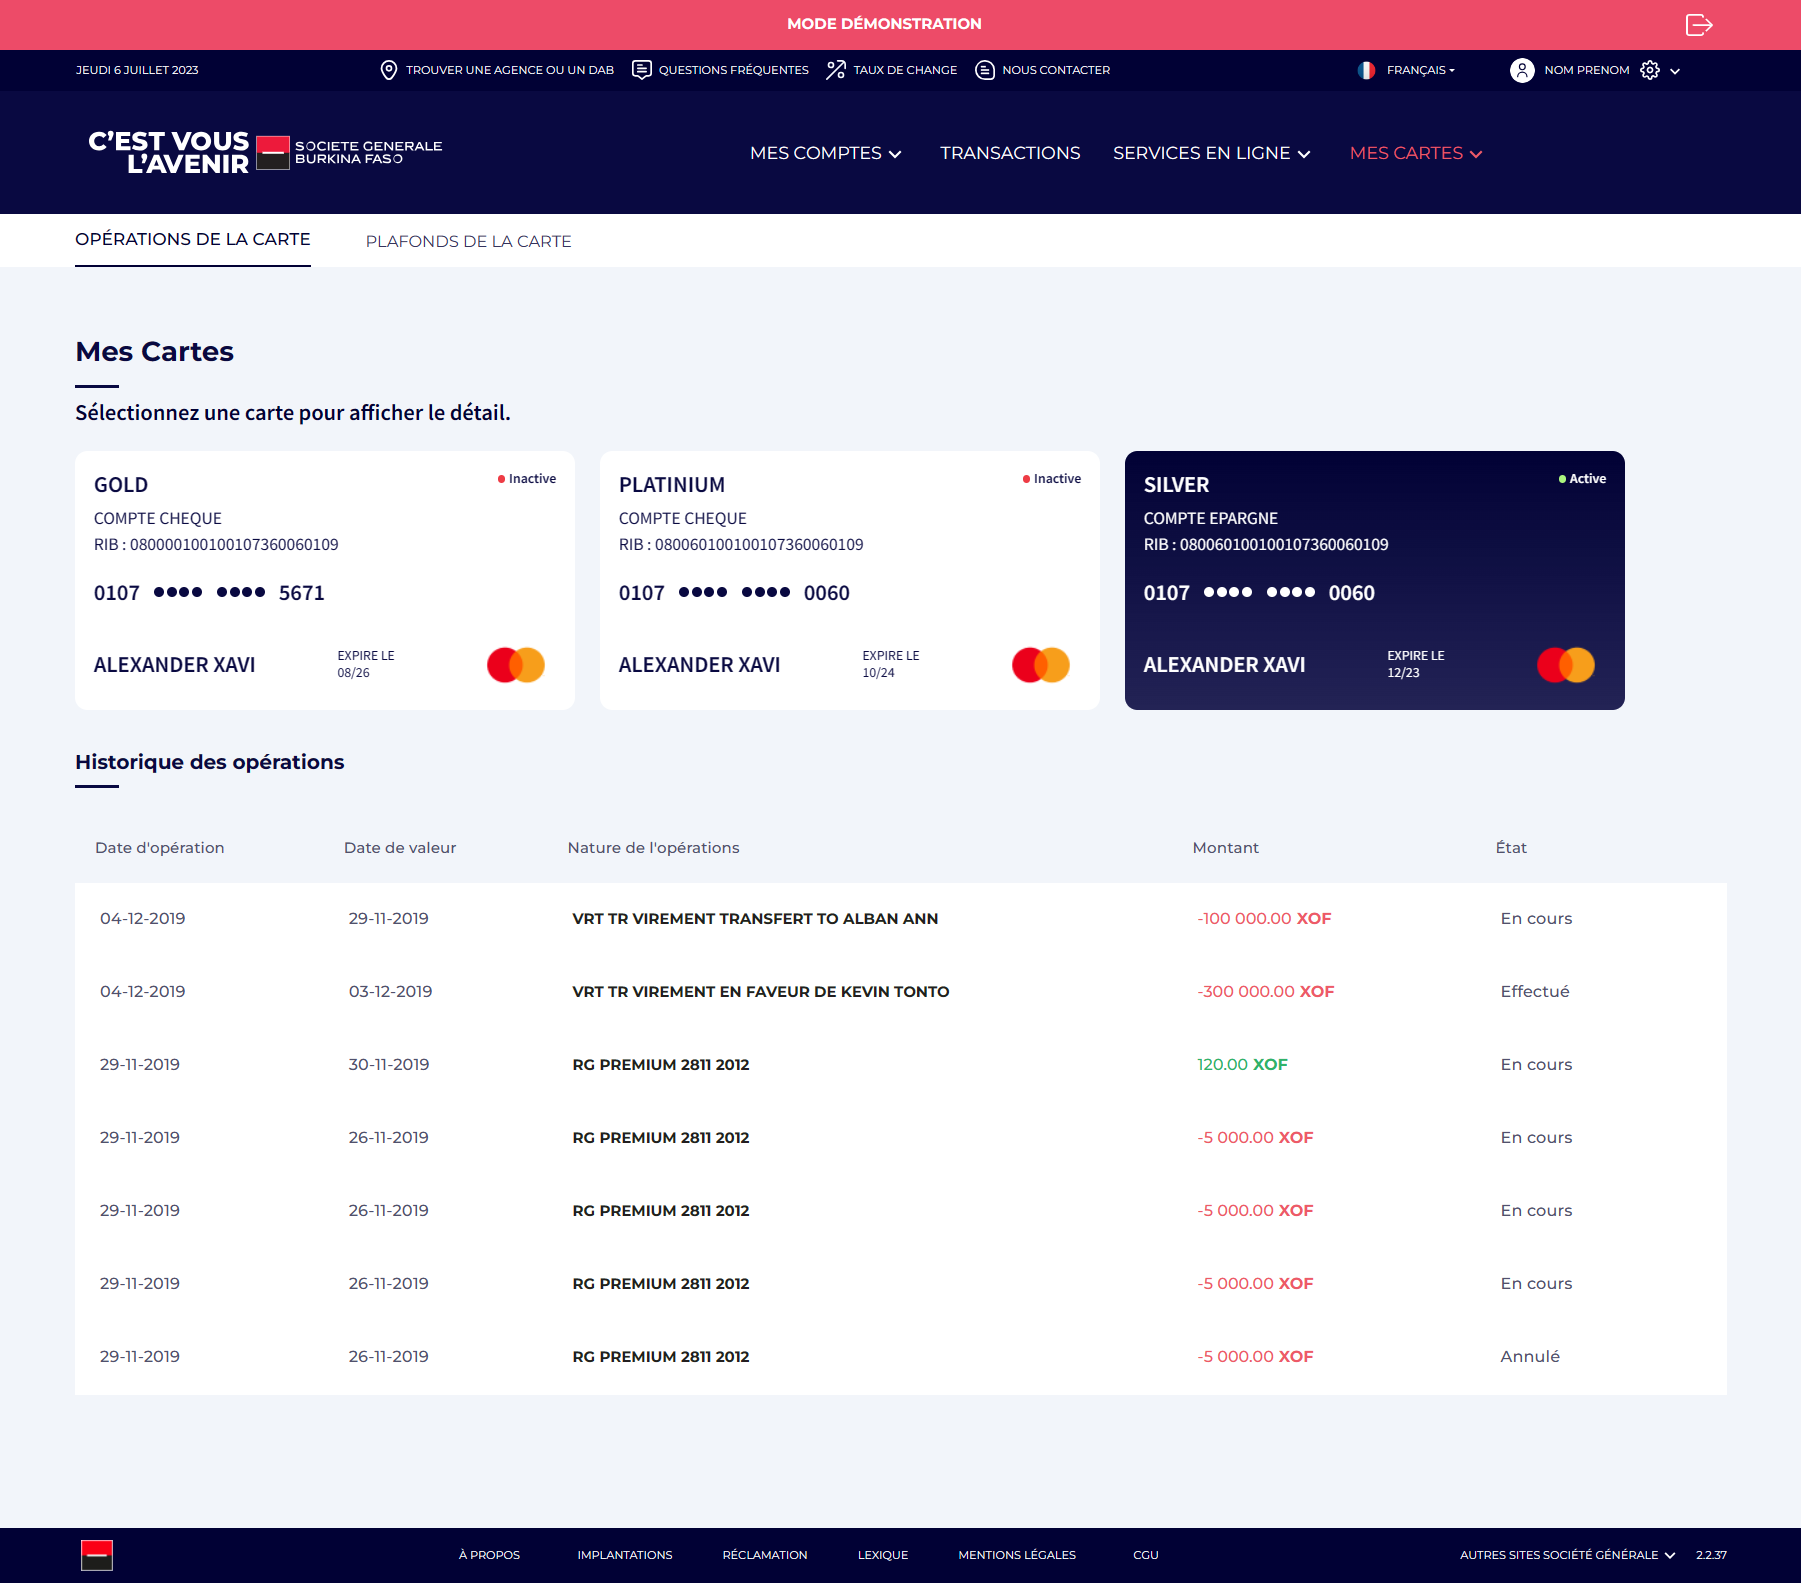
\includegraphics[width=\textwidth]{images/screens/cartes/desktop.png}
        \caption{version française}
    \end{subfigure}
    \hfill
    \begin{subfigure}[b]{0.49\textwidth}
        \centering
        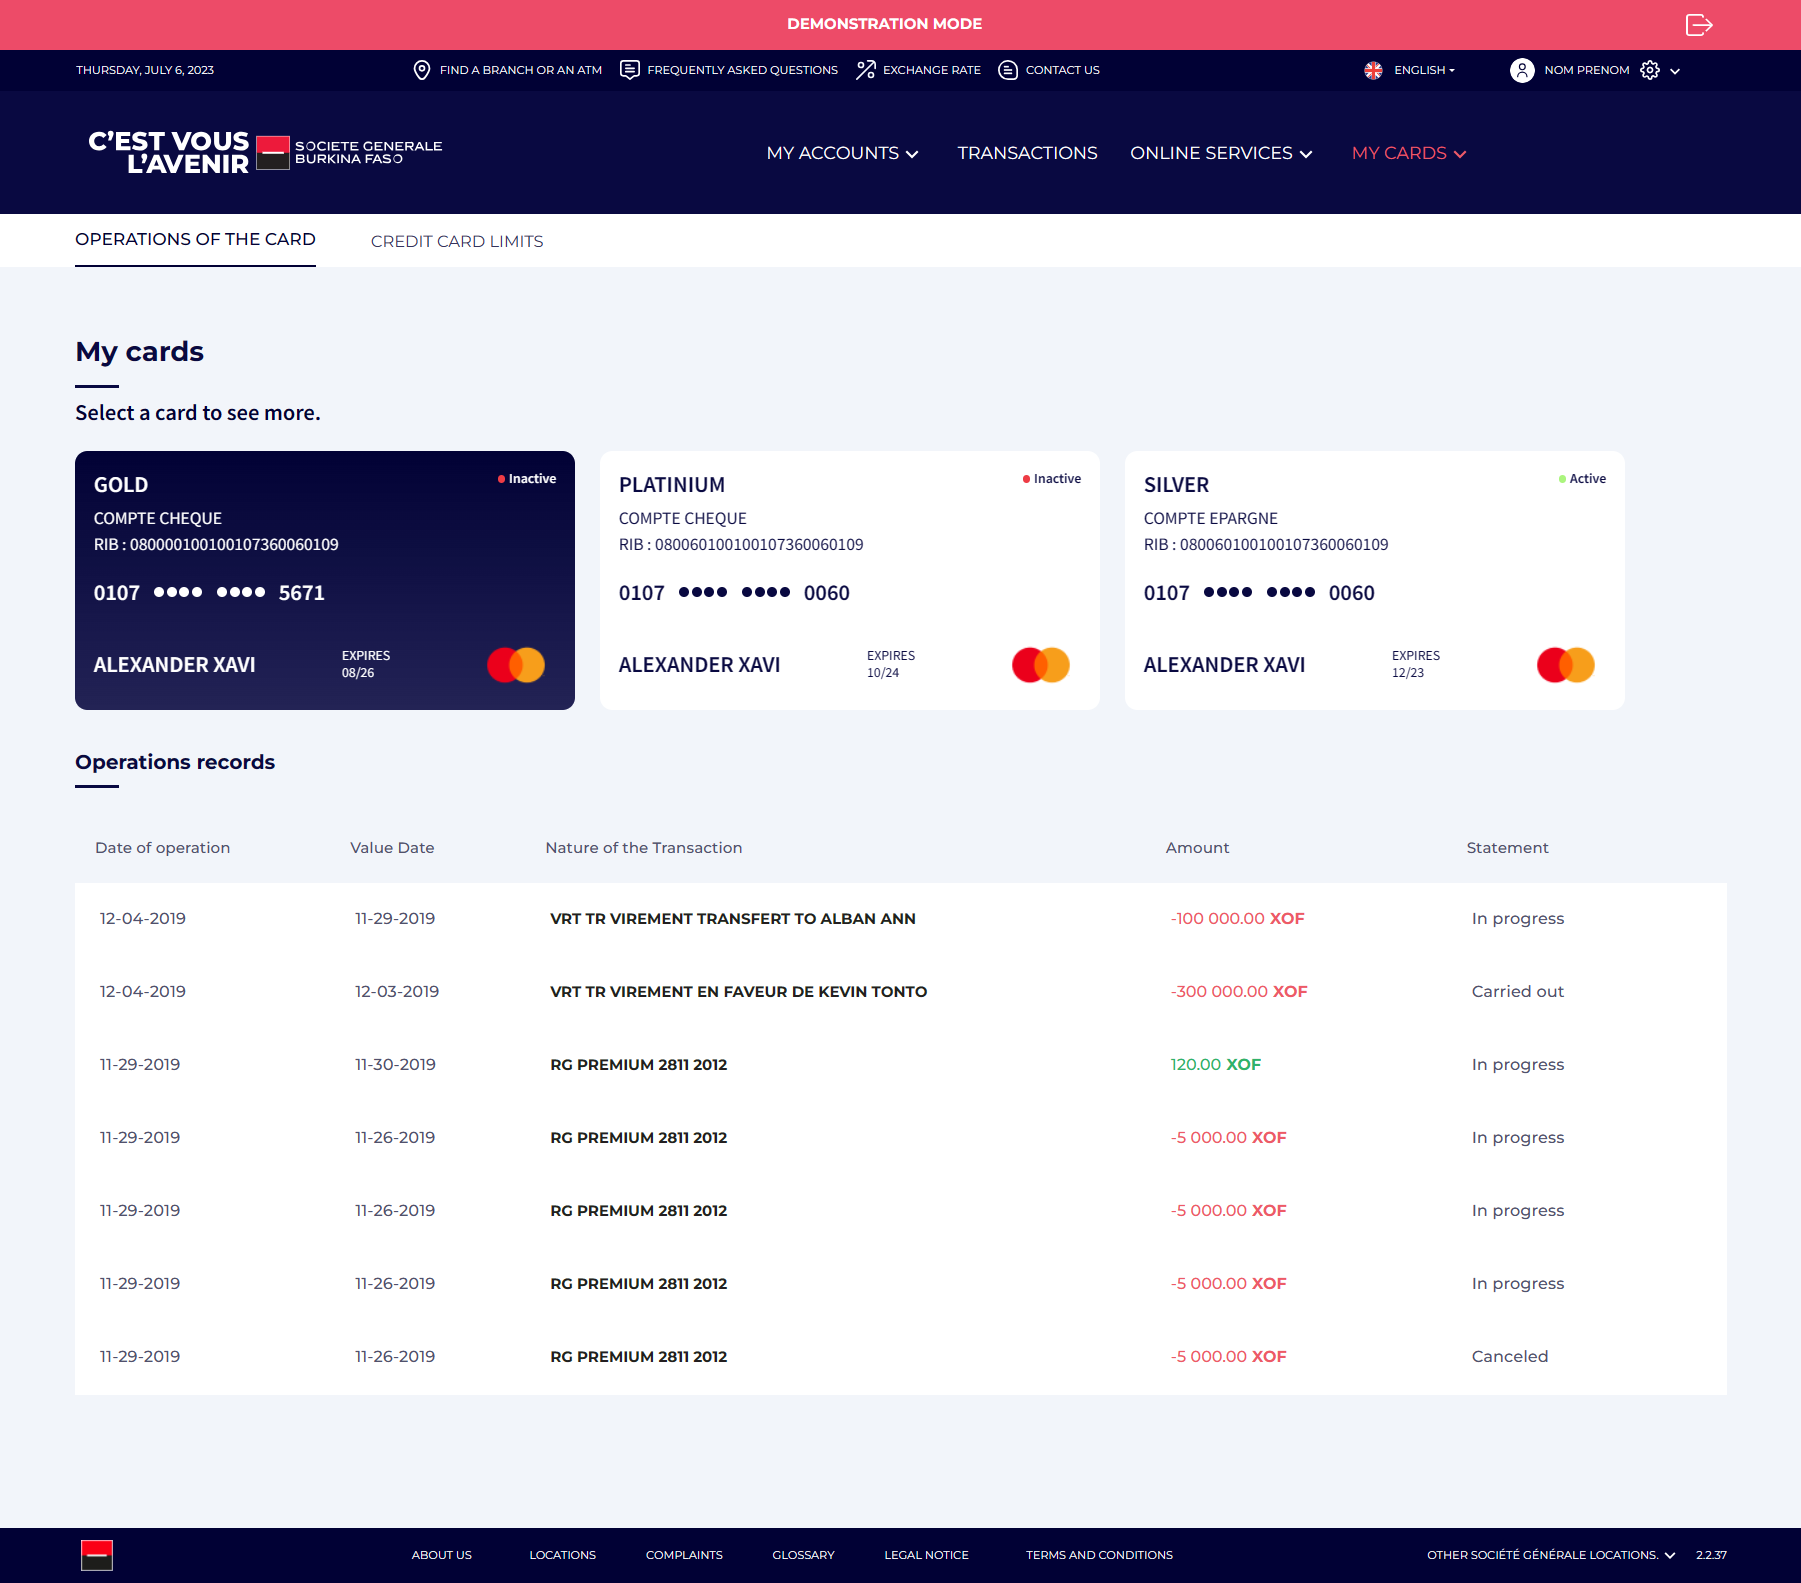
\includegraphics[width=\textwidth]{images/screens/cards/desktop.png}
        \caption{version anglaise}
    \end{subfigure}
       \caption{Interface Mes cartes sur le bureau}
\end{figure}

\newpage

\begin{figure}[!ht]
    \centering
    \begin{subfigure}[b]{0.49\textwidth}
        \centering
        \includegraphics[width=\textwidth]{images/screens/cartes/tablette.png}
        \caption{version française}
    \end{subfigure}
    \hfill
    \begin{subfigure}[b]{0.49\textwidth}
        \centering
        \includegraphics[width=\textwidth]{images/screens/cards/tablette.png}
        \caption{version anglaise}
    \end{subfigure}
       \caption{Interface Mes cartes sur la tablette}
\end{figure}

\newpage


\begin{figure}[!ht]
    \centering
    \begin{subfigure}[b]{0.49\textwidth}
        \centering
        \includegraphics[width=\textwidth]{images/screens/cartes/mob.png}
        \caption{version française}
    \end{subfigure}
    \hfill
    \begin{subfigure}[b]{0.49\textwidth}
        \centering
        \includegraphics[width=\textwidth]{images/screens/cards/mob.png}
        \caption{version anglaise}
    \end{subfigure}
       \caption{Interface Mes cartes sur le mobile}
\end{figure}

\newpage

\begin{figure}[!ht]
    \centering
    \begin{subfigure}[b]{0.49\textwidth}
        \centering
        \includegraphics[width=\textwidth]{images/screens/mobileApp/device/Cards Home D.png}
    \end{subfigure}
    \hfill
    \begin{subfigure}[b]{0.49\textwidth}
        \centering
        \includegraphics[width=\textwidth]{images/screens/mobileApp/device/Cards Details D.png}
    \end{subfigure}
       \caption{Interface Mes cartes sur l'application mobile}
\end{figure}

\newpage

\begin{figure}[!ht]
    \centering
    \begin{subfigure}[b]{0.49\textwidth}
        \centering
        \includegraphics[width=\textwidth]{images/screens/cartes/mob-button.png}
        \caption{version française}
    \end{subfigure}
    \hfill
    \begin{subfigure}[b]{0.49\textwidth}
        \centering
        \includegraphics[width=\textwidth]{images/screens/cards/mob-button.png}
        \caption{version anglaise}
    \end{subfigure}
       \caption{Bouton pour voir plus de détails sur la transaction}
\end{figure}

\newpage

\begin{figure}[!ht]
    \centering
    \begin{subfigure}[b]{0.49\textwidth}
        \centering
        \includegraphics[width=\textwidth]{images/screens/cartes/mob-details.png}
        \caption{version française}
    \end{subfigure}
    \hfill
    \begin{subfigure}[b]{0.49\textwidth}
        \centering
        \includegraphics[width=\textwidth]{images/screens/cards/mob-details.png}
        \caption{version anglaise}
    \end{subfigure}
       \caption{Détails de la transaction}
\end{figure}

\newpage

\begin{figure}[!ht]
    \centering
    \begin{subfigure}[b]{0.49\textwidth}
        \centering
        \includegraphics[width=\textwidth]{images/screens/mobileApp/device/Cards Transactions Details D.png}
    \end{subfigure}
       \caption{Détails de la transaction dans l'application mobile}
\end{figure}

\subsection{Plafonds des cartes}
L'interface "Plafonds des cartes" offre une vue claire et détaillée des limites nationales et internationales de chaque carte.\\

Grâce à l'API \textbf{getCardLimits}, les données sont récupérées en temps réel pour assurer que les informations affichées sont toujours à jour.
\newpage
\subsubsection*{Plafonds nationaux}
\begin{figure}[!ht]
    \centering
    \begin{subfigure}[b]{0.49\textwidth}
        \centering
        \includegraphics[width=\textwidth]{images/screens/plafondsNat/desktop.png}
        \caption{version française}
    \end{subfigure}
    \hfill
    \begin{subfigure}[b]{0.49\textwidth}
        \centering
        \includegraphics[width=\textwidth]{images/screens/limitsnat/desktop.png}
        \caption{version anglaise}
    \end{subfigure}
       \caption{Interface Plafonds nationaux sur le bureau}
\end{figure}

\begin{figure}[!ht]
    \centering
    \begin{subfigure}[b]{0.49\textwidth}
        \centering
        \includegraphics[width=\textwidth]{images/screens/plafondsNat/tablette.png}
        \caption{version française}
    \end{subfigure}
    \hfill
    \begin{subfigure}[b]{0.49\textwidth}
        \centering
        \includegraphics[width=\textwidth]{images/screens/limitsnat/tablette.png}
        \caption{version anglaise}
    \end{subfigure}
       \caption{Interface Plafonds nationaux sur la tablette}
\end{figure}

\newpage

\begin{figure}[!ht]
    \centering
    \begin{subfigure}[b]{0.49\textwidth}
        \centering
        \includegraphics[width=\textwidth]{images/screens/plafondsNat/mob.png}
        \caption{version française}
    \end{subfigure}
    \hfill
    \begin{subfigure}[b]{0.49\textwidth}
        \centering
        \includegraphics[width=\textwidth]{images/screens/limitsnat/mob.png}
        \caption{version anglaise}
    \end{subfigure}
       \caption{Interface Plafonds nationaux sur le mobile}
\end{figure}
\newpage

\begin{figure}[!ht]
    \centering
    \begin{subfigure}[b]{0.49\textwidth}
        \centering
        \includegraphics[width=\textwidth]{images/screens/mobileApp/device/Cards Limits D.png}
    \end{subfigure}
    \begin{subfigure}[b]{0.49\textwidth}
        \centering
        \includegraphics[width=\textwidth]{images/screens/mobileApp/device/Cards Limits Details D.png}
    \end{subfigure}
       \caption{Interface Plafonds nationaux sur l'application mobile}
\end{figure}

\newpage

\subsubsection*{Plafonds internationaux}
\begin{figure}[!ht]
    \centering
    \begin{subfigure}[b]{0.49\textwidth}
        \centering
        \includegraphics[width=\textwidth]{images/screens/plafondsInter/desktop.png}
        \caption{version française}
    \end{subfigure}
    \hfill
    \begin{subfigure}[b]{0.49\textwidth}
        \centering
        \includegraphics[width=\textwidth]{images/screens/limitsInter/desktop.png}
        \caption{version anglaise}
    \end{subfigure}
       \caption{Interface Plafonds internationaux sur le bureau}
\end{figure}

\begin{figure}[!ht]
    \centering
    \begin{subfigure}[b]{0.49\textwidth}
        \centering
        \includegraphics[width=\textwidth]{images/screens/plafondsInter/tablette.png}
        \caption{version française}
    \end{subfigure}
    \hfill
    \begin{subfigure}[b]{0.49\textwidth}
        \centering
        \includegraphics[width=\textwidth]{images/screens/limitsInter/tablette.png}
        \caption{version anglaise}
    \end{subfigure}
       \caption{Interface Plafonds internationaux sur la tablette}
\end{figure}
\newpage

\begin{figure}[!ht]
    \centering
    \begin{subfigure}[b]{0.49\textwidth}
        \centering
        \includegraphics[width=\textwidth]{images/screens/plafondsInter/mob.png}
        \caption{version française}
    \end{subfigure}
    \hfill
    \begin{subfigure}[b]{0.49\textwidth}
        \centering
        \includegraphics[width=\textwidth]{images/screens/limitsInter/mob.png}
        \caption{version anglaise}
    \end{subfigure}
       \caption{Interface Plafonds internationaux sur le mobile}
\end{figure}
% \newpage

\subsection{Mes Produits}
L'interface "Mes produits" permet aux utilisateurs de consulter les différents produits bancaires souscrits pour un compte spécifique. Cette fonctionnalité offre une vue d'ensemble complète des engagements financiers associés à chaque compte, tels que les crédits, les prêts ou les services d'investissement.\\

Grâce à l'API \textbf{getAccountProducts}, les données sont récupérées en temps réel pour assurer que les informations affichées sont toujours à jour. Les utilisateurs peuvent visualiser les détails de chaque produit, y compris les caractéristiques, les conditions d'utilisation et les dates d'échéance.

\begin{figure}[!ht]
    \centering
    \begin{subfigure}[b]{0.49\textwidth}
        \centering
        \includegraphics[width=\textwidth]{images/screens/produits/desktop.png}
        \caption{version française}
    \end{subfigure}
    \hfill
    \begin{subfigure}[b]{0.49\textwidth}
        \centering
        \includegraphics[width=\textwidth]{images/screens/products/desktop.png}
        \caption{version anglaise}
    \end{subfigure}
       \caption{Interface Mes produits sur le bureau}
\end{figure}
\newpage

\begin{figure}[!ht]
    \centering
    \begin{subfigure}[b]{0.49\textwidth}
        \centering
        \includegraphics[width=\textwidth]{images/screens/produits/tablette.png}
        \caption{version française}
    \end{subfigure}
    \hfill
    \begin{subfigure}[b]{0.49\textwidth}
        \centering
        \includegraphics[width=\textwidth]{images/screens/products/tablette.png}
        \caption{version anglaise}
    \end{subfigure}
       \caption{Interface Mes produits sur la tablette}
\end{figure}
\newpage

\begin{figure}[!ht]
    \centering
    \begin{subfigure}[b]{0.49\textwidth}
        \centering
        \includegraphics[width=\textwidth]{images/screens/produits/mob.png}
        \caption{version française}
    \end{subfigure}
    \hfill
    \begin{subfigure}[b]{0.49\textwidth}
        \centering
        \includegraphics[width=\textwidth]{images/screens/products/mob.png}
        \caption{version anglaise}
    \end{subfigure}
       \caption{Interface Mes produits sur le mobile}
\end{figure}


\subsection{Téléchargement du récapitulatif}
Les utilisateurs ont la possibilité de télécharger le récapitulatif d'un produit spécifique auquel ils ont souscrit. Pour ce faire, il leur suffit de cliquer sur le bouton "Télécharger le récapitulatif" associé au produit concerné.\\

\begin{figure}[!ht]
    \centering %
        \includegraphics[width=16cm]{images/screens/produits/desktop-button.png}
    \caption{Bouton de téléchargement du récapitulatif}
\end{figure}

Lorsque l'utilisateur clique sur ce bouton, notre application génère automatiquement le récapitulatif du produit souscrit et le propose en téléchargement. Le fichier téléchargé contient toutes les informations pertinentes sur le produit, telles que les détails de souscription, les termes et conditions, les fonctionnalités, et tout autre élément pertinent lié au produit.
\begin{figure}[!ht]
    \centering %
        \includegraphics[width=16cm]{images/screens/produits/Récapitulatif.png}
    \caption{Exemple d'un récapitulatif de produit}
\end{figure}
\newpage

\section{Environnements de déploiement}
Les stratégies de déploiement suivies dans notre projet sont différentes selon l’environnement de
déploiement. Les environnements adoptés par la DIFA sont :

\begin{itemize}
    \item[•] \textbf{LOCAL :} L’environnement LOCAL est utilisé par les développeurs sur leurs propres machines
    pour le développement et les tests. Ils disposent d’une installation locale du système et des outils
    nécessaires. Cela leur permet de travailler de manière autonome et de tester les fonctionnalités
    dans un environnement contrôlé.
    \item[•] \textbf{Development [DEV] :} Il s’agit du premier niveau de machines individuelles, à ce stade l’application est hébergée dans un ou plusieurs agents Nomad dans une ou plusieurs machines virtuelles
    fonctionnant dans des centres de données cloud privés, seuls les développeurs y ont accès pour
    valider la fonctionnalité de leur application lors de l’exécution.
    \item[•] \textbf{Homologation Fonctionnelle [HF] :} Tout comme le DEV, cet environnement est hébergée dans un agent Nomad avec des informations d’identification et des données stockées en toute sécurité,
    ces données diffèrent de celle de l’environnement DEV car elles doivent communiquer avec d’autres
    instances d’autres systèmes, cet environnement est créé pour que les Business Analyst, les Proxy
    Product Owner et les Product Owner puissent y exécuter les tests d’acceptation et valider le comportement de l’application.
    \item[•] \textbf{Homologation Technique [HT] :} Également appelé ISO-PROD, ce qui signifie qu’il a exactement les mêmes caractéristiques que l’environnement de production. Il permet de tester l’application dans un environnement de type production, et valider qu’elle supporte la charge de travail,
    les critères du système et tout incident technique pouvant survenir en production.
    \item[•] \textbf{Production [PROD] :}  A ce stade l’application est entièrement testée et validée pour être accessible aux clients, elle est également dupliquée dans plusieurs instances, différentes machines
    physiques, et aussi différentes régions géographiques pour assurer une disponibilité permanente
    possible.
\end{itemize}

\section{Qualification}
La phase de qualification comprend différents tests qui garantissent la qualité et la fiabilité du
système. Parmi ces tests, on retrouve les tests end-to-end, les tests fonctionnels et les tests de
non-régression.

\subsection{Tests end to end}
Les tests end-to-end, réalisés en environnement local sont réalisés pour vérifier le fonctionnement
global du système, en simulant des scénarios réels de bout en bout. Ils permettent de valider
l’intégration des différents composants et de s’assurer que toutes les fonctionnalités interagissent
correctement.
\begin{figure}[!h]
    \centering %
        \includegraphics[width=16cm]{images/realisation/cypressLanguage.png}
    \caption{Exemple de test end to end en utilisant Cypress}
\end{figure}
\newpage

\subsection{Tests fonctionnels}
Les tests fonctionnels, réalisés en environnement HF, se concentrent sur la vérification des fonctionnalités individuelles du système. Ils permettent de valider que chaque fonctionnalité répond
aux exigences spécifiées et fonctionne comme prévu.
\subsection{Tests de non regression}
Les tests de non-régression, réalisés en environnement HT, sont effectués pour s’assurer que les
modifications apportées au système n’ont pas introduit de régressions, c’est-à-dire qu’elles n’ont pas affecté négativement les fonctionnalités existantes. Ces tests garantissent la stabilité du système
lors de l’ajout de nouvelles fonctionnalités ou de modifications.

\section{Perspectives}  
Nous identifions plusieurs fonctionnalités qui peuvent être développées dans le cadre futur du projet de banque en ligne. Bien que ces fonctionnalités n'aient pas encore été implémentées, elles représentent des opportunités d'amélioration et d'extension du système. Les principales perspectives sont les suivantes :

\begin{itemize}
    \item[•] \textbf{Modification des plafonds :}  Une fonctionnalité clé à envisager est la possibilité pour les utilisateurs de modifier les plafonds de leurs cartes. Cela permettrait aux clients d'ajuster les limites de dépenses et de retraits en fonction de leurs besoins et de leurs préférences, offrant ainsi une plus grande flexibilité et un meilleur contrôle sur leurs transactions financières.
    \item[•] \textbf{Développement de la page "Store" :} Une autre perspective intéressante est la création d'une page dédiée au "Store" où les utilisateurs peuvent découvrir et consulter les produits financiers proposés par les banques partenaires. Cette fonctionnalité permettrait aux clients d'avoir une vision plus complète et transparente des offres disponibles, favorisant ainsi une prise de décision éclairée pour leurs besoins bancaires.
    \item[•] \textbf{Déploiement :}  Le déploiement est une étape essentielle pour rendre le système de banque en ligne accessible aux clients finaux. Cette perspective implique le déploiement de l'application sur des serveurs ou des infrastructures adaptés, permettant ainsi une utilisation réelle par les utilisateurs. Un déploiement réussi garantirait une disponibilité et une stabilité optimales de l'application pour une expérience utilisateur fluide et fiable.
\end{itemize}

\section{Conclusion}
Le chapitre "Réalisation et mise en œuvre" a été une étape clé dans notre projet de développement de la banque en ligne. Nous avons réussi à concrétiser les spécifications et les besoins identifiés lors de l'étude détaillée du projet, en mettant en place les interfaces, les fonctionnalités et les environnements nécessaires.
